\documentclass[a4paper, 12pt]{article}
\usepackage{outlines}
\usepackage{graphicx}
%\usepackage{times}
\usepackage{xcolor}
\usepackage{float}
\usepackage{mathtools}
\usepackage{enumerate}
\usepackage{geometry}
\usepackage[english]{babel}
\usepackage{array}
\usepackage{wrapfig}
\usepackage{amsmath}
\usepackage{multirow}
\usepackage{tabu}
\usepackage{titlesec}
\usepackage{titletoc}
\usepackage{array}



\titleformat{\section}[display]%
{\null\fontsize{16}{5}\rmfamily\bfseries\filcenter}{CAPITOLUL \thesection}{1em}{}[]
\titleformat{name = \section, numberless}[block]%
{\null\fontsize{16}{5}\rmfamily\bfseries\filcenter}{}{1em}{}
\titlespacing*{\section}{0em}{1em}{1em}

\titlecontents{section}
[7em] % ie, width of contentslabel + 0.5em
{\medskip}
{\contentslabel[\MakeUppercase\chaptername~\thecontentslabel]{7.5em}}%\thecontentslabel
{\hspace*{-6.5em}}
{\titlerule*[0.5pc]{.}\contentspage}

\addto{\captionsenglish}{
	\renewcommand{\refname}{Referințe bibliografice}%
	\renewcommand{\contentsname}{Cuprins}
	\renewcommand{\listfigurename}{Lista imaginilor}
}
\addto\captionsenglish{\renewcommand{\chaptername}{Capitolul}}
%define the page geometry
\geometry{
	a4paper,
	left=25mm,
	top=25mm,
	bottom=25mm,
	right=25mm,
}
\renewcommand{\baselinestretch}{1.5}
\makeatletter
\renewcommand\paragraph{\@startsection{paragraph}{4}{\z@}%
	{-2.5ex\@plus -1ex \@minus -.25ex}%
	{1.25ex \@plus .25ex}%
	{\normalfont\normalsize\bfseries}}
\makeatother
\setcounter{secnumdepth}{4} % how many sectioning levels to assign numbers to
\setcounter{tocdepth}{4}    % how many sectioning levels to show in ToC



\begin{document}

%define the title page
\begin{titlepage}
	\begin{center}
		\vspace{0.5cm}
		\LARGE \textsc{Universitatea "Babeș Bolyai"}
		\LARGE \textsc{Cluj-Napoca}
		\\
		\vspace{0.5cm}
		\Large \textsc{Facultatea de studii europene}
		\\
		\Large \textsc{Specializare Management}
		
		
		\vspace{1.5cm}
		
		\Huge Comportamentul consumatorului online roman tanar si educat - Studiu de caz
		\\
		\bigskip
	

		\vspace{0.5cm}		
		\Large LUCRARE DE LICENȚĂ
		
		\vfill
		
		\Large
		\textsc{Coordonator}\hfill \textsc{Autor}
		\\
		\large
		\textsc{Conf. dr. Nicoleta RACOLȚA-PAINA}\hfill\textsc{CIUCANU Sorina}
		
		\vspace{1.5cm}
		\textsc{Cluj-Napoca, România}\\
		\textsc{Iulie 2021}
		
	\end{center}
\end{titlepage}
\restoregeometry

%put the table of contents
\tableofcontents

%put the list of figures
\newpage
\listoffigures

%this section is on new page
\newpage
\nocite{bobalcua2015loyal}
\nocite{london_economics_2011}
\nocite{duralia2016particularities}
\nocite{devderea2018consumer}
\nocite{armstrong2014principles}
\nocite{orzan2014study}
\nocite{obradattitudes}
\nocite{sava_2020}
\nocite{bighiu2015compulsive}
\nocite{gorunescu_2020}

\section*{Declaratie}
\newpage

\section*{Introducere}
\addcontentsline{toc}{section}{\textsc{Introducere}}
	
	\quad\quad Lucrarea de fata " Comportamentul consumatorului online roman, tanar si educat" abordeaza un subiect vast si de actualitate care devine din ce in ce mai important pentru firmele care doresc sa-si dezvolte strategii de marketing axate pe factorii ce determina consumatorul online sa aleaga un producator in detrimentul altuia. Din pacate nu exista multe studii pe tema procesului de cumparare a consumatorului online din Romania, ci doar articole din alte tari atat din Uniunea Europeana cat si din afara acesteia. Precizam ca aceasta lucrare pune accentul pe consumatorul  individual si nu pe cel organizational (entitati juridice) deoarece dorim sa analizam ce anume determina cumparatorul individual sa achizitioneze produse care sunt de larg consum.
	
	\quad Scopul prezentei lucari de licenta este realizarea unui profil al consumatorului onlin tanar si educat din Romania pentru ca firmele din comertul electronic sa inteleaga mai bine comportamentul acestuia si sa se plieze pe nevoile si dorintele lui.
	
	\quad Prezentul studiu isi propune sa prezinte principalele aspecte teoretice si practice cu privire la comportamentul consumatorilor online respectiv practice referitoarea la factorii care influenteaza comportamentul consumatorului online roman,tanar si educat, pentru ca in final sa oferim informatii de folos companiilor ce practica comertul electronic si sunt prezente pe piata din Romania.
	
	\quad La fel ca orice demers stintiific, este nevoie de existenta unei baze teoretice care sa vina in ajutorul analizei informatiilor obtinute in urma studiului de caz. Astfel, pentru partea teoretica este utilizata cartea fondatorului marketing-ului, Philip Koetler, articole de la Comisia Europeana privind la nivel de Uniune consumatorul online, dar si cateva articole de la autori romani precum Duralia Oana de la Universitatea Lucian Blaga din Sibiu si Claudia Bobalca care si-au manifestat interesul fata de perceptia consumatorilor asupra bunurilor online. 
	
	\quad Partea practica reprezinta o cercetare primara cantitativa, metoda folosita fiind sondajul de opinie, iar instrumentul de culegere a datelor fiind chestionarul(lansat online in perioada 27.04.-04.05) .	Chestionarul folosit (vezi Anexa 1) cuprinde 3 intrebari filtru si anume una legata de varsta( intervalul ales de noi fiind 18-30), o alta leagata de nivelul de studii(minim BAC)si respectiv numarul de achizitii online, cu plata card in februarie-aprilie 2021(aici dorind sa avem raspunsuri de la consumatorii avizati). Am ales ca respondentii sa aiba un anumit interval de varsta si anume 18-30 deoarece in domeniul marketing-ului este necesara pozitionarea si segmentarea pietei tinta.
	
	\quad Structura lucrarii include atat o sectiune teoretica cat si o sectiune practica, avand in total un numar de 4 capitole. Primul capitol, numit "Comportamentul consumatorului online - continut si tendinte" cuprinde 6 subcapitole dar si 5 subsubcapitole in care se discuta la modul general de consumatorul online. Astfel, prima parte a capitolului cuprinde o introducere a subiectului si anumite bariere ce se regasesc in mediul digital. Pe urma, lucrarea pune accent pe consumatorul online incepand cu formularea unui scurt profil al acestuia, apoi cu trend-uri prezente in cererea cumparatorilor, continuand cu factori care tind sa influenteze decizia de cumparare a acestuia, procesul de cumparare impartit si detaliat pe etape si in cele din urma, avantajele si dezavantajele pe care consumatorii online le-au intalnit si depasit in experientele lor in mediul online. 
	
	\quad Al doilea capitol, numit "Cercetare secundara privind comportamentul constumatorului online, tanar si educat din Romania" cuprinde 4 subcapitole. Primul subcapitol releva informatii despre comertul electronic din Romania oferind statistici despre cumparaturilor online ale romanilor,categoriile de produse care sunt cumparate cel mai frecvent online de populatia din Romania si contextul actual al pandemiei Covid19 care a avut o influenta puternica asupra achizitiilor online. Urmatoarele subcapitole includ trei perspective asupra achizitiilor online, studii de caz ce ofera informatii despre comportamentul consumatorului online, tanar si educat din Romania, iar la final o scurta concluzie a celor trei articole.
	
	\quad Lucrarea continua cu al treilea capitol, care cuprinde cercetarea propriu-zisa si reprezinta esenta prezentei lucrari stiintifice deoarece realizeaza conexiunea intre elementele teoretice cuprinse in capitolele anterioare si modul in care se aplica acestea in practica. Astfel, dupa cum am mentionat anterior, in elaborarea acestui capitol este utilizat o metoda de cercetare cantitativa (instrumentul folosit fiind chestionarul) pentru a obtine informatiile necesare atingerii obiectivelor propuse si anume, crearea unui profil al consumatorului online, tanar si educat din Romania.
	
	\quad Lucrarea prezinta o serie de limitari ca urmare a lipsei surselor bibliografice si studiilor datorat numarului scazut de cercetari asupra comportamentului consumatorului online din Romania. De asemenea, reticienta respondentilor de a raspunde la chestionar, in special a respondentilor de genul masculin, mi-a ingreunat munca in cercetarea mea cantitativa. Un aspect neasteptat a fost numarul mare de respondenti care au ales la intrebarea filtru referitoare la numarul minim de achizitii online in perioada februarie-aprilie 2021 mai putin de 5 achizitii online, fapt ce m-a determinat sa nu includ in cercetarea mea o mare parte din totalul de respondenti.
	
	\quad Luand in considerare cele afirmate mai sus, exprimam speranta ca aceasta cercetare aduce un plus de valoare pentru domeniul teoretic, referitor la comportamentul consumatorului online, tanar si educat din Romania si implicarea sa in comertul electronic.
		
\newpage
\setcounter{section}{0}
\section{ Comportamentul consumatorului online - conținut și tendințe}

\subsection{Comertul electronic}
\quad \quad\space În ultimii zece ani, in contextul internațional al comunicării digitale, comerțul electronic devine o importantă parte a sistemului de afaceri. Odată ce Internetul a devenit un instrument foarte utilizat si important în comunicare, promovare și tranzacții comerciale, noi platforme s-au dezvoltat pentru a crea strategii competitive. Ca sa putem fi mai clari, voi defini comerțul electronic drept orice formă de tranzacție comercială unde părțile implicate interacționeaza într-un mod electronic.\footnote{Claudia Bobalca, "The Loyal Customers’ Perception Regarding The Online
	Buying Process", \textit{Central and Eastern European Online Library}, Economie, p.241, https://www.ceeol.com/search/article-detail?id=282663, data accesarii: 29.03.2021}

\quad 
Intr-o economie globala dezvoltata intr-o piata foarte competitiva, orientarea spre consumator nu mai reprezinta doar un trend ci o necesitate pentru companii sa obtina succes. Astfel, o buna intelegere a modului in care consumatorii beneficiaza de proprietatile Internetului, factorii pe care ii iau in considerare pentru a se hotara asupra deciziilor de cumparare in mediul comertului electronic, aduce avantaje semnificative pentru managerii care doresc sa dezvolte strategii de marketing potrivite profilului consumatorilor pe care ii au. Cumparatorii online au acces nelimitat la informatie si au oportunitatea de a alege dintr-o gama larga de optiuni in selectarea produselor si serviciilor potrivite acestora.

\quad In acest caz, merita remarcat faptul ca comertul electronic include ambele tipuri de tranzactii implicand atat bunuri tangibile precum electronice, bunuri de larg consum, jucarii care trebuie sa fie livrate fizic catre consumator, dar si tranzactii privind accesul la bunuri intangibile, precum sevicii sau produse care pot fi furnizate digital catre consumator. De asemenea, trebuie mentionat faptul ca exista bunuri care se gasesc atat in format electronic cat si in format fizic precum cartile, revistele, muzica si jocurile.

\quad In urma experientelor privind achizitia unor produse/servicii online, unii consumatori au intalnit si cateva bariere care i-a determinat sa evite mediul digital, printre care principalele le enumaram mai jos:
\begin{itemize}
	\item Potrivit rezultatelor de la Eurostat cel mai frecvent motiv pe care consumatorii l-au mentionat a fost preferinta pentru cumparaturi in format fizic sau faptul ca nu simt nevoia de a utiliza mediul online pentru a plasa comenzi.
	\item Un alt motiv foarte des intalnit, pe care il mentioneaza informatiile de la Eurostat, sunt riscurile privind securitatea, intimitatea si grijile privind increderea in a-si impartasi datele personale pe care consumatorii le intampina atunci cand doresc sa plaseze o comanda online.
	\item De asemenea, consumatorii au adaugat ca lipsa sau insuficienta informatiilor despre un anumit produs i-a determinat sa evite achizitiile unor bunuri online.\footnote{European Parliament, "Consumer behaviour in a digital environment", p.77, data accesarii : 29.03.2021}
\end{itemize}

	\quad Acceptarea de catre consumator a internetului drept un mijloc de informare, comparare de informatii  si cumparare a diverse bunuri si servicii a rezultat in ceea ce literatura de specialitate defineste prin conceptul de e-consumator sau consumator electronic.\footnote{Oana Duralia, "Particularities of the european consumer`s behaviour in online environments", p.21, data accesarii : 29.03.2021}  Spre deosebire de consumatorii traditionali, care sunt mai conservatori si mai constanti in alegerile lor, e-consumatorii manifesta o deschidere mai mare pentru schimbare, fiind mult mai disponibili sa incerce lucruri noi.\footnote{Ibidem} In plus, daca ar fi sa cream un portret al e-consumatorului l-am putea descrie drept o persoana inovativa, creativa, educata, cu studii superioare si cu un status socio-economic ridicat.
	

	\subsection{Factori care influenteaza consumatorul online}
	\qquad\space Avand in vedere dezvoltarea tehnologiei de-a lungul ultimilor ani,  paradigma achizitiilor a schimbat modul in care cumparatorii isi pot achizitiona diverse bunuri, incurajandu-se acum mai mult ca niciodata consumul. Astfel, consumatorul contemporan face fata la mult mai multe provocari legate de lipsa de timp, multitudinea de optiuni si volumul de informatii disponibile pentru a putea lua o decizie privind procurarea unui produs. Diversi autori au venit cu diferite abordari si studii privind factorii care ar putea influenta decizia de cumpararea a unui e-consumator in zilele noastre.
	
	\quad O abordare foarte interesanta este reprezentata de autorul Paul Henry, care exemplifica constrangerile care afecteaza comportamentul consumatorului de-a lungul procesului de cumparare online (figure 1).
	\begin{figure}[!htb]
		\centering
		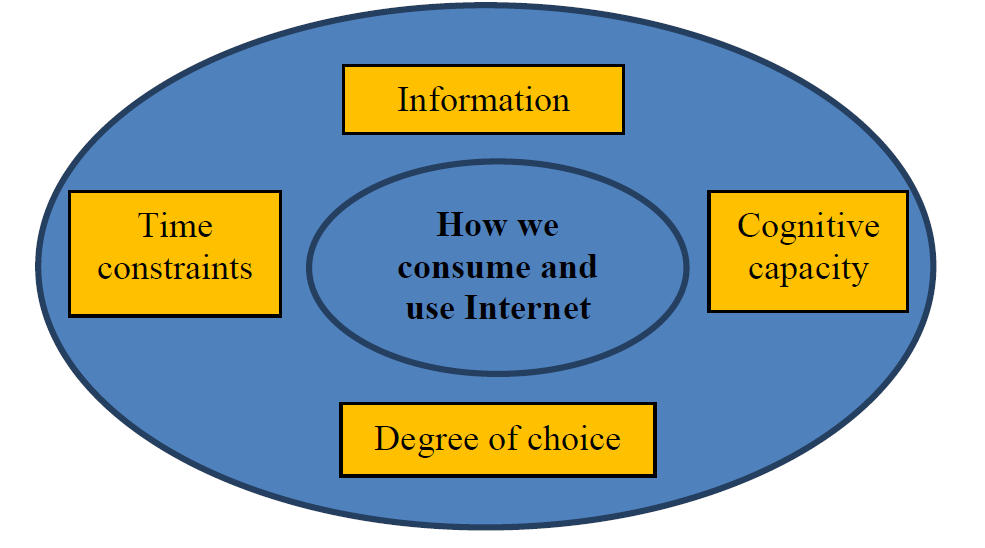
\includegraphics[width=13cm, height=8cm]{"figures/first.png"}
		\caption{Factori de constrangere in procesul de cumparare al consumatorului}\label{fig:first}
	\end{figure}

	\quad Dupa cum se observa si in figura, impactul celor patru factori mentionati deasupra sunt foarte cunoscuti si relativ usor de inteles; Ne aflam intr-o perioada in care cumparatorul este afectat de presiunea timpului, considerata drept o resursa limitata si rara pe care trebuie sa o foloseasca, sa se informeze prin diverse canale media pentru a reusi, in cele din urma, sa faca cele mai bune alegeri dintre optiunile pe care le ofera piata. Marea provocare ramane modul in care consumatorul reuseste sa analizeze, interpreteze si sa integreze informatia obtinuta (abilitatea cognitiva) si sa o transforme in cunostinte utile si valoroase.\footnote{Ibidem, p. 23}
	
	\quad O alta abordare asupra factorilor care influenteaza achizitiile online ale consumatorilor apartine profesorilor Ujwala Dange and Vinay Kimar( figure 2) care au creat modelul "FFF".  
	\begin{figure}[!htb]
		\centering
		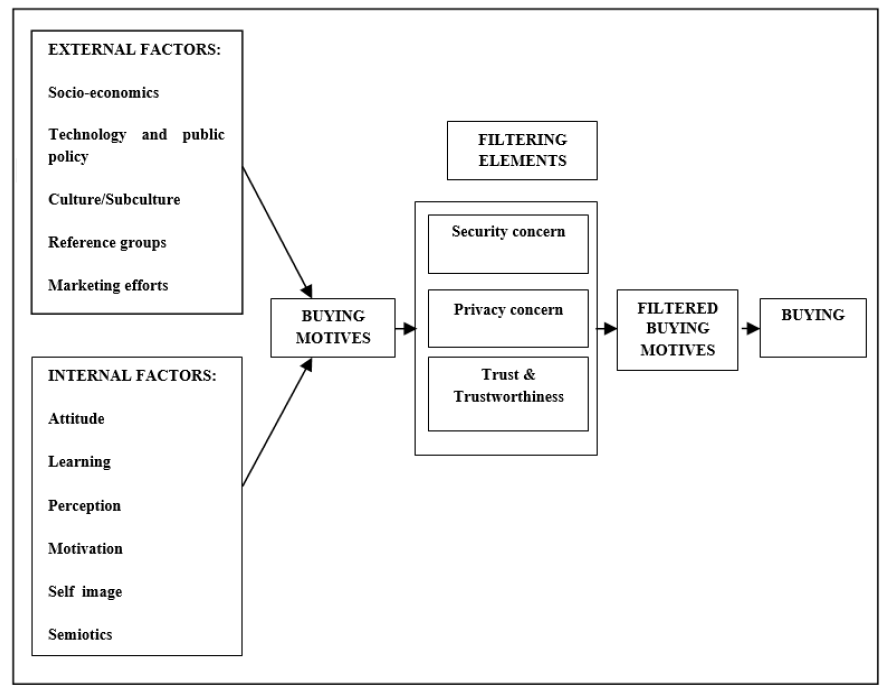
\includegraphics[width=15cm, height=12cm]{"figures/SECOND.png"}
		\caption{Modelul FFF al comportamentului consumatorului online}\label{fig:second}
	\end{figure}

	Acest model porneste de la cele trei categorii de influente exercitate asupra comportamentului cumparatorului in mediul online si anume: factori interni si externi care pot provoca cumparatorul sa plaseze comenzi online; factorii de filtrare a informatiilor prin prisma riscului perceput de cumparatorul online si factorii de filtrare a deciziilor de cumparare, in legatura cu modul in care consumatorul isi evalueaza propriile asteptari si motive drept un rezultat al actiunii tuturor influentelor mentionate mai sus.\footnote{Ibidem, p.24}
	
	\quad Spre deosebire de abordarea autorului Paul Henry privind impedimentele care ar putea ingreuna procesul de cumparare si abordarea profesorilor Ujwala Dange si Vinay Kimar, cu modelul celor trei tipuri de factori, se adauga abordarea lui Ciprian Devderea care, in urma cercetarii perspectivelor pe care alti autori le au asupra factorilor care influenteaza decizia cumparatorului de a achizitiona sau nu un produs online, a remarcat trei mari elemente care se evidentiaza si care ajuta consumatorul sa faca alegerea potrivita.\footnote{Ciprian Devderea, "Consumer Behavior Towards Apparel E-Commerce in Romania", p.473-475 }
	\begin{itemize}
		\item\textbf{Calitatea paginii web si anxietatea tehnologica} 
		
		\quad O mare importanță în comerțul electronic este calitatea web. Pe lângă faptul că are un rol funcțional, calitatea web-ului sau designul site-ului web pot afecta percepția consumatorului și pot influența dacă consumatorul este mulțumit sau nu de ambianță. In plus, accesibilitatea si usurinta folosirii paginii web va determina daca consumatorul va reveni sa mai achizitioneze si alte produse sau va renunta din cauza unor elemente care ii ingreuneaza plasarea unei comenzi online precum neorganizarea produselor pe categorii, lipsa unor poze reprezentative a bunului achizitionat, solicitarea de prea multe informatii personale, etc.
		
		\quad Cu toate acestea, dincolo de calitatea experienței online, anxietatea este un subiect frecvent abordat în contextul comportamentului consumatorului online. Anxietatea tehnologică, în contextul cumpărăturilor online, este o reacție negativă care îi influențează pe utilizatori să se îndoiască de capacitatea lor de a efectua o anumită acțiune sau de a-și reduce așteptările cu privire la rezultat.\footnote{Ibidem} Acest lucru inseamna ca utilizatorii au noi griji atunci cand achizitioneaza online, anumite categorii de produse. Un exemplu relevant sunt cumparaturile online de imbracaminte, in acest caz consumatorii online trebuie sa ia in considerare noi elemente precum diferenta de dimensiune, diferitele unitati de masurare si alte detalii mici care pot transforma placerea cumparatorilor de a achizitiona intr-un stres din cauza incertitudinii.
		
		\item\textbf{Securitatea si confidentialitatea}
		
		\quad Aceste doua elemente sunt exprimate prin increderea pe care consumatorii o au in achizitionare unor bunuri online. Astfel, exista diverse studii care confirma importanta securitatii si confidentialitatii informatiilor personale pe care consumatorii trebuie sa le ofere in momentul in care plaseaza o comanda. Din pacate, multi consumatori evita magazinele online tocmai din cauza acestor doi factori care le genereaza o atitudine negativa fata de mediul digital fie din cauza lipsei de experienta a consumatorului sau a unor experiente neplacute din trecut. Insa, in prezent, exista reglementari clare si stricte privind drepturile consumatorului online, care au rolul de a oferi utilizatorilor o anumita siguranta.
		
		\item\textbf{Online Word of Mouth} 
		
		\quad Conceptul de Word of Mouth in contextul comertului electronic(e-WOM) se refera la o conversație online între utilizatori despre un produs sau experiență, care de obicei poate fi negativă sau pozitivă.\footnote{Ibidem}. Pentru a intelege mai bine, pot oferi un exemplul tot in contextul cumpararii de imbracaminte online, amintit anterior. In acest caz, se poate lua in considerare actul de interactiune dintre doi utilizatori care vorbesc despre experienta lor de a comanda un anumit produs de la un anumit magazin online. Astfel, in acest proces, are loc un transfer de informatii care vor influenta negativ sau pozitiv decizia de a achizitiona din viitor de la acel furnizor online.
		
	\end{itemize}

	\subsection{Procesul de cumparare al consumatorului online}
		\quad\quad Dupa ce am discutat despre lucrurile ce ar putea sa determine un consumator sa achizitioneze sau nu un produs vom vedea procesul care sta la baza deciziei pe care acesta trebuie sa o ia. In primul rand, trebuie sa mentionam ca in teoria economica traditionala, consumatorul trebuie sa actioneze ca un individ rational cand vine vorba de achizitia unui bun sau a unui serviciu, punand in balanta costurile si beneficiile ce i se aduc, alegand cea mai buna optiune care ii satisface complet nevoile.
		
		\quad La baza analizei comportamentului consumatorului online sta procesul decizional al cumparatorului impartit pe etapele ilustrate in figura 3.\footnote{Eurpean Parliament, \textit{op. cit}, p.38}
		\begin{figure}[!htb]
			\centering
			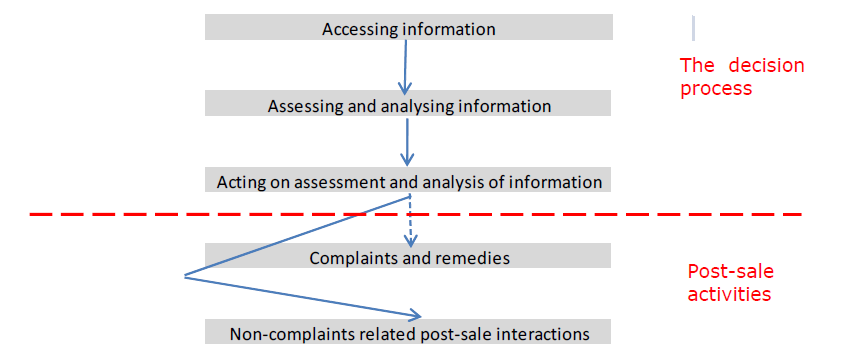
\includegraphics[width=12cm, height=7cm]{"figures/third.png"}
			\caption{Procesul de cumparare al conumatorului online}\label{fig:third}
		\end{figure}
	
		\subsubsection{Accesarea informatiei}
		\quad\quad
		 In momentul in care un consumator incepe sa se gandeasca la  achizitionarea unui bun, in spatele acestei dorinte sta nevoia pentru un obiect specific sau pentru anumite calitati ale acelui produs sau serviciu. Astfel, in aceasta etapa, el incepe sa consulte toata informatia la care poate avea acces pentru a o rezuma si conclude intr-o decizie.\footnote{Koetler \& Armstrong, "Principles of Marketing 14th edition, p.153}
		
 		\quad In mediul digital, s-au creat de-a lungul dezvoltarii tehnologice diverse motoare de cautare pentru facilitarea gasirii de informatii oferind consumatorilor diverse platforme ce comercializeaza produsele de care e interesat, insa, pe de alta parte, volumul mare de date disponibil online este considerat de unii consumatori drept coplesitor.
		 
	 	\quad De asemenea, consumatorii se bazeaza  si pe  retelele de socializare drept un furnizor de informatii folositoare pentru decizia lor de cumparare deoarece acolo regasesc review-uri si recomandari de la persoane pe care ei le cunosc si le considera de incredere.\footnote{Orzan Gheorghe, Boboc Larisa- Andreea, Burghelea Ioana, Stupu Diana Luana, "A STUDY OF ONLINE USER’S BEHAVIOUR TOWARDS FACEBOOK SOCIAL NETWORK", 2014, p.3}
		
		\subsubsection{Evaluarea si analiza informatiei }
		
		\quad\quad Dupa ce consumatorul a adunat toata informatia disponibila online, acesta incepe sa analizeze optiunile pe care le are dupa factorii care reprezinta o importanta pentru el precum brand-ul, calitatea, pretul, reputatia produsului etc., si in cele din urma sa aleaga ce tip de produs/ serviciu doreste si de la ce producator sa-l achizitioneze. \footnote{Koetler \& Armstrong, \textit{op. cit}}
		
		\quad Neutilizand instrumente de filtrare si sortare a informatiei, consumatorii tind sa ia in considerare doar primele cautari ce le apar in topul listei, uneori bazandu-se pe brand-urile pe care ei deja le cunosc in locul celor noi aparute pe piata si netestate inainte fizic.
		
		\quad Cu toate ca internetul ofera o multitudine de elemente referitoare la produsele disponibile pe magazinele web, unele produse nu contin detaliile semnificative cu privire la componenta lor. Astfel, consumatorii, neavand posibilitatea de a atinge sau mirosi produsele inainte de a le cumpara, evita produsele pe care nu le-au incercat in magazinul fizic, deoarece implica o evaluare mult mai dificila a informatiei descoperite online.
		
		\quad Se remarca, de asemenea, faptul ca in ciuda volumului mare de informatii despre anumite produse sau servicii, sursa de incredere pe care se bazeaza cel mai mult consumatorii atunci cand vine vorba de evaluarea unui produs nou, neincercat, raman recomandarile si parerile persoanelor apropiate sau experienta proprie din trecut.
		
		\subsubsection{Luarea deciziei}
		
		\quad\quad In aceasta etapa consumatorul a inteles nevoia care trebuie sa fie satisfacuta, a parcurs toate si analizat informatiile necesare luarii unei decizii si urmeaza sa-si plaseze comanda online de la producatorul care reuseste sa indeplineasca toate criteriile care prezinta relevanta si importanta pentru cumparator.
		
		\quad  Comertul electronic ii ofera cumparatorului diverse avantaje precum o varietate larga de produse, posibilitatea de a plati un pret mai mic pe un produs ce se regaseste si in magazinul fizic, dar si unele riscuri precum utilizarea datelor personale pentru alte scopuri  fara consimtamantul lor si frica de costurile extra, ascunse, strategie folosita de unele firme si cunoscuta drept "drip-pricing".\footnote{European Parliament, \textit{op.cit} p.52}
		
		\subsubsection{Mecanismul de reclamatii si recurs}
		
		\quad\quad Este necesar de mentionat ca aceasta etapa se aplica numai atunci cand consumatorul are o problema cu produsul sau serviciul livrat si vrea sa faca o reclamatie catre producator. Procesul de cumparare intr-o piata digitala difera de procesul consumatorului offline care achizitioneaza din magazinul fizic, unde are posibilitatea de a observa si analiza toate calitatile si defectele unui anumit bun. Prin urmare, atunci cand cumparatorii achizitioneza in mediul online e posibil ca ei sa experimenteze o schimbare in tipul si magnitudinea problemei pe care o intalnesc fata de cele in magazinele fizice, implicand de asemenea riscuri mai mari.
		
		\quad Se considera ca un consumator rational s-ar plange catre vanzator daca intampina o problema cu produsul sau serviciul livrat insa, in realitate nu toti cumparatorii aleg sa revina cu un feedback si sa faca o sesizare despre defectele surprise, din diverse motive personale, iar acest lucru este si mai dificil intr-un mediul online spre deosebire de cel fizic.\footnote{Ibidem, p.90}
		
		\quad In mare parte din problemele pe care un consumator le poate experimenta in momentul in care plaseaza o comanda online au legatura cu  modul de livrarea si cu calitatea promisa pe care descrierea de pe site sugereaza ca o detine un anumit produs si care in momentul primirii coletului se denota contrariul asteptarilor.
		
		\subsubsection{Serviciile si interactiunile post-vanzare}
		
		\quad\quad Unii producatori apeleaza la interactiunile si serviciile post-vanzare intre cumparator si firma pentru a crea o legatura de lunga durata care il va determina pe consumator sa mai plaseze si alte comenzi in viitorul apropiat.\footnote{Ibidem, p.98} Aceste strategii de promovare, consta in comunicarea de promotii la pachete de produse, reduceri disponibile pe site-ul web, vouchere periodice pentru fidelizarea clientilor etc. Cu toate ca aceste oferte ar putea suna atractive la prima vedere, unii consumatori considera ca trimiterea unor astfel de email-uri, fara permisiunea lor, poate fi considerata drept o initiativa time consuming si care creeaza iritare.
		
		\quad\subsection{Trend-uri in comportamentul consumatorilor online} 
		Un studiu al Comisiei Europene a observat/identificat cateva trend-uri prezente in cererea consumatorilor care au distins numeroasele faciltati datorate posibilitatii de a plasa comenzi pe Internet:\footnote{Ibidem, p.21}
		\begin{itemize}
			\item \textbf{Civilizarea si mobilizarea consumului} care implica faptul ca e-consumatorii consuma din ce in ce mai mult de acasa sau chiar si cand sunt pe drum. In plus, mai exista un trend care implica ca plasarea de comenzi nu are loc numai unde cumparatorul doreste dar si la ce ora considera el. Aceste trenduri sunt facilitate de noi tehnologii precum reteaua de internet si serviciile de pe telefon la care ai acces 24 de ore pe zi, facand posibil utilizatorilor sa plaseze comenzi oricand au placerea si nevoia.
			\item \textbf{Globalizarea} care afecteaza nu numai productia internationala cat si cererea globala. Consumatorii asteapta acum produse din toata lumea sa fie livrate la usa casei. Tehnologiile de informare si comunicare au facut ca comertul dintre diverse tari sa fie foarte accesibil iar toti consumatorii din orice parte a lumii sa aiba acces la cat mai multe produse similare.
			\item \textbf{Personalizarea}, spre deosebire de productia in masa amintita anterior, drept componenta a globalizarii, pune accent pe particularizarea produselor si serviciilor la nevoile individuale ale fiecarui cumparator astfel incat sa aduca un plus valoare acelui bun pentru a crea avantaje competitive.
		\end{itemize}
		
		\subsection{Avantajele achizitiei online}
		
		\quad\quad De-a lungul experientelor consumatorilor privind achizitiile in mediul online s-au remarcat diverse avantaje care i-a determinat pe consumatori sa paseasca in piata digitala pentru a-si satisface nevoile sau dorintele personale. Printre acestea enumeram: 
		\begin{itemize}
			\renewcommand{\labelitemi}{$\Rightarrow$}
			\item Oportunitatea de a plati preturi mai mici deoarece in mediul digital magazinele online platesc costuri mai mici fata de magazinele fizice, de exemplu chiria.
			\item  Accesul la o varietate mai mare de produse si producatori. Acest lucru reprezinta o importanta mare pentru zonele sarace in care nu sunt atat de dezvoltate magazinele clasice.
			\item Posibilitatea de a achizitiona un bun la orice ora si oriunde doreste consumatorul in limita stocului disponibil de pe site.
			\item Cresterea usurintei comparatiei caracteristicilor produselor cu ajutorul anumitor platforme sau chiar compararea aceluiasi produs dar de la diferiti producatori.
			\item Abilitatea de a  oferi si de a primi recomandari si pareri care pot ajuta consumatorii sa ia o decizie asupra procesului de cumparare al unui anumit bun.
		\end{itemize}
	
		\subsection{Dezavantajele achizitiei online}
		
		\quad\quad Cu toate ca dezvoltarea pietelor de desfacere a dus la extinderea lor si in mediul digital iar majoritatea consumatorilor au inceput sa fie atrasi mai mult de beneficiile cumpararii de pe platforme online, unii cumparatori au intampinat si probleme care i-a determinat sa se gandeasca de doua ori atunci cand doresc sa plaseze o comanda online. Printre aceste probleme s-au remarcat: 
		\begin{itemize}
			\renewcommand{\labelitemi}{$\Rightarrow$}
			\item Non-livrarea sau intarzierea livrarii unui produs care mentiona ca ajunge intr-un anumit interval de timp si a depasit cu mult timpul de asteptare. 
			\item Bunurile care nu s-au prezentat la momentul livrarii conform caracteristicilor afisate pe site-ul producatorului.
			\item Diverse probleme referitoare la garantia unor produse cum ar fi in cazul electronicelor care au garantie pe o perioada mai mare de timp.
			\item  Bunuri care la momentul deschiderii ambalajului aveau defecte iar producatorul nu avea o politica de return privind produsele cu probleme.
			\item Riscurile privind securitatea si protectia datelor personale furnizate necesare livarii la domiciliul consumatorului a produsului sau serviciului.
			\item Costurile sau preturile care nu sunt afisate complet pe anumite site-uri ale producatorilor.
		\end{itemize}
	\newpage
\section{Cercetare secundara privind comportamentul consumatorului online, roman, tanar si educat}
	\subsection{Comertul electronic in Romania}
	\qquad  În România, piața de comerț electronic și-a făcut prezența la inceputul anului 2004\footnote{Obrad Ciprian, Vasile Gherghes, "ATTITUDES TOWARDS ONLINE COMMERCE: A CASE STUDY OF STUDENT POPULATION IN TIMIȘOARA", 2016, p.47} și a început să se dezvolte cu adevărat cu admiterea țării în Uniunea Europeană atunci când fondurile europene pentru investițiile în infrastructură au început să fie accesibile. Chiar dacă acest lucru a fost un beneficiu pentru dezvoltarea comerțului electronic în România și în prezent conform statisticilor naționale, 55,8\% din gospodăriile din România au un computer la domiciliu (INS 2013) și 54,4\% din gospodării atât în zonele rurale, cât și în cele urbane au acces la Internet, rata cumpărăturilor online rămâne destul de scăzută în Europa de Est, inclusiv în România (INS 2014). In cele din urma, decizia de a cumpăra online este, de asemenea, influențată si de factorii culturali (Lim et al., 2004).\footnote{Onete, C. B., Teodorescu, I. and Vasile, V., 2016. "Considerations Regarding the Analysis of the Digital Consumer in Romania. Amfiteatru Economic", p. 656}
	
	\qquad Comerțul electronic a devenit din ce în ce mai prezent pe lista românilor de opțiuni de cumpărături, în contextul unei rate de penetrare a internetului în creștere: "Deși penetrarea pe Internet în România este încă scăzută în comparație cu media europeană de 70\%, până în 2018, ratele sunt asteptate să fie semnificativ mai echilibrate cu peste două treimi din populația care are acces la domiciliu la Internet "(Euromonitor, 2014).\footnote{Claudia Bobalca, \textit{op.cit}, p.241}
	
	\quad Privind contextul achizitiilor online, românii cumpără în cea mai mare parte electronice și jocuri video, îmbrăcăminte, produse de frumusete si produse de ingrijire personala. Cu tot mai mulți clienți care trec la cumpărăturile online și o rată în continuă creștere a prezenței online a comercianților cu amănuntul pe piața românească, o mare provocare pentru manageri, este de a atrage noi clienți, formând  totodata și clienți loiali.\footnote{Ibidem, p.242} Cu cat exista mai mult acces la informații și având deja o experiență de cumpărare, obiceiurile de cumpărături online ale românilor sunt în continua dezvoltare. Noua generație de tineri este mai familiarizată cu tehnologia online, are mai multă experiență în utilizarea internetului și este mai dispusa să se confrunte cu riscurile percepute de achizitiile online.
	
	\quad Un alt factor important care a favorizat achizitiile online in ultima perioada este pandemia Covid19 care a afectat intreaga lume, inclusiv Romania.\footnote{Claudia Gorunescu, Ecommerce in timpul convid-19: Ce impact resimte piata din Romania, accesat in data de: 25.04.2021} Astfel, multi antreprenori romani s-au mutat in mediul online pentru a-si putea salva afacerile din cauza restrictiilor impuse pentru protejarea cetatenilor si a consumatorilor.
	 Exista date statistice care sublinieaza o crestere a cumparaturilor online in randul romanilor in aceasta perioada precum figura 4 de mai jos care arata o comparatie intre frecventa cumpararaturilor online inainte, in timpul si dupa pandemia Covid19.\footnote{Statista 2021, https://www.statista.com/statistics/1169383/romania-online-shopping-frequency/, accesat in data de 15.04.2021.}
	 	\begin{figure}[!htb]
	 	\centering
	 	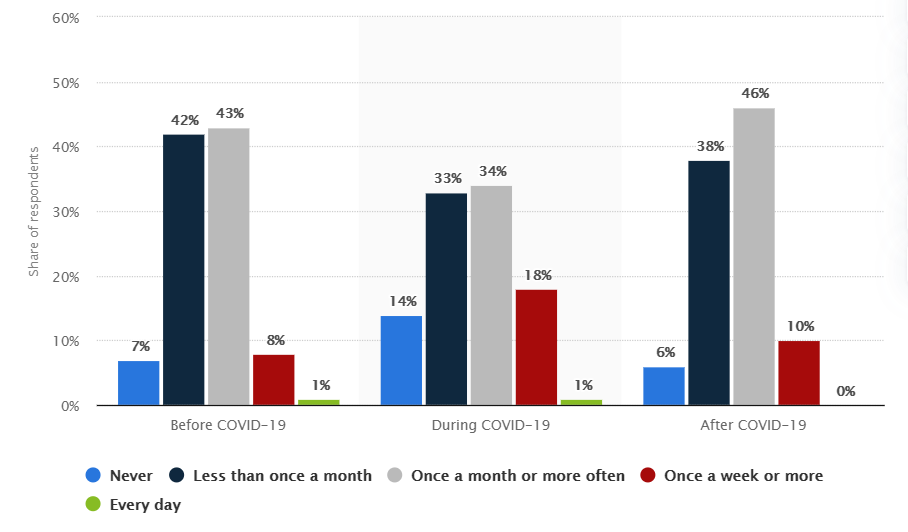
\includegraphics[width=13cm, height=9cm]{"figures/fourth.png"}
	 	\caption{ Frecventa cumparaturilor online in Romania 2020-2021}\label{fig:fourth}
		 \end{figure}
 
 \qquad Pentru a aduce informatii noi privind comportamentul consumatorilor online tineri si educati din Romania a fost necesar parcurgerea a mai multor articole care furnizau date despre ecommerce-ul din Romania. In cele din urma, trei articole s-au evidentiat deoarece detineau drept subiect comportamentul consumatorului online si tanar din Romania cu varste cuprinse intre 18-35 de ani. Am impartit cele trei articole in trei studii caz A, B si C oe care le voi face prezenta pe scurt prin prisma elementelor prin care se diferentiaza si prin informatiile noi aduse despre comportamentul consumatorului online tanar si educat din Romania.
 \subsection{Cercetarea A}
 Studiul de caz "A" este scris in 2016 si publicat in Amfiteatrul Economic  de trei autori: Cristian Bogan Onete, Ioana Teodorescu si Viorel Vasile; Articolul surprinde o analiza asupra componentelor comportamentului consumatorului digital din Romania in contextul evolutiei cumparaturilor online. Studiul incepe cu informatii generale despre nivelul comertul electronic la nivel de Uniune Europeana, la nivel de tara si aduce un plus de valoare cu  factori predominanti care influenteaza alegerea unui consumator roman inainte de a achizitiona online afisati in tabelul din figura 5.\footnote{Onete, C. B., Teodorescu, I. and Vasile, \textit{op.cit}}
 	\begin{figure}[!htb]
 	\centering
 	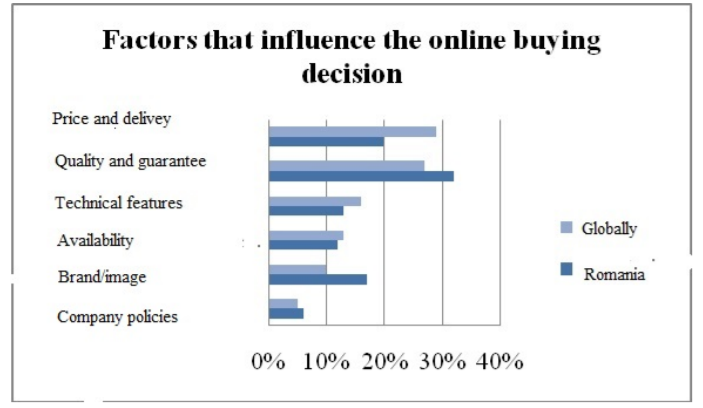
\includegraphics[width=12cm, height=7cm]{"figures/fifth.png"}
 	\caption{Factori care influenteaza decizia de cumparare online a romanilor}\label{fig:fifth}
 \end{figure}

		\quad  Potrivit acestui tabel am descoperit că consumatorii digitali români sunt influențați cel mai mult de calitatea și garantarea unui produs / serviciu (32\% în România, 27\% la nivel global). În România, cel mai important factor pare a fi calitatea și garanția unui produs, în timp ce respondenții la nivel global sunt influențați cel mai mult prin preț și livrare (29\%), după cum se poate observa în figura 5. Termenii de preț și de livrare se situează pe locul doi în opinia respondenților români (20\% în România, 29\% la nivel global), în timp ce marca / imaginea este, de asemenea, un factor decisiv pe care consumatorii îl iau în considerare (17\% în România, 10\% la nivel global ).
		
		\quad Scopul principal al lucrării este de a înțelege comportamentul românesc digital al consumatorilor incepand cu motivul pentru care românii preferă să cumpere produse / servicii pe piețele externe pe Internet si pana la identificarea factorilor care influenteaza comportamentul consumatorului. Metoda de preluare a datelor a fost un chestionar electronic administrat la 160 de utilizatori de social media, din mediul urban, educati, cu varste cuprinse intre 20-35 de ani.
		
		\quad Conform rezultatelor, chestionarul a fost completat 74\% de femei si 26\% de barbati. Printre intrebarile sondajului, s-a evidentiat intrebarea 3 care arata pietele principale comerciale online de la care romanii achizitioneaza online, afisate in figura 6. 
		\begin{figure}[!htb]
			\centering
			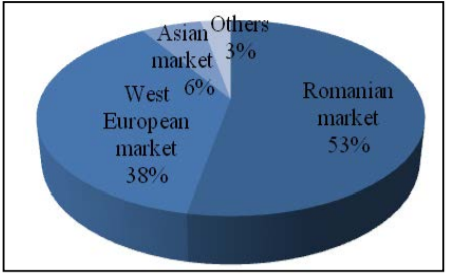
\includegraphics[width=10cm, height=7cm]{"figures/sixth.png"}
			\caption{Online markets}\label{fig:sixth}
		\end{figure}
	
	\qquad O alta intrebare relevanta comportamentului consumatorului online din Romania a fost motivul pentru care romanii cumpara de la producatori din afara tarii.
	\begin{figure}[!htb]
		\centering
		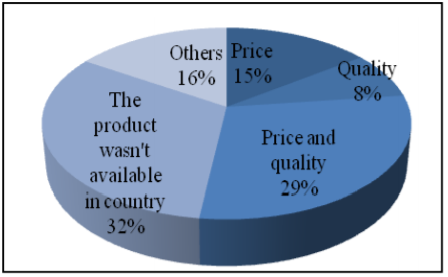
\includegraphics[width=10cm, height=7cm]{"figures/seventh.png"}
		\caption{Motive pentru a cumpara de la producatori straini}\label{fig:seventh}
	\end{figure}

	\quad Ultima intrebare relevanta arata categoriile de produse pe care consumatorii online din Romania le cumpara de la producatorii din strainatate in mod frecvent, afisate de asemenea, prin figura 8 reprezentativa a rezultatelor. Acest lucru denota faptul ca românii își satisfac nevoile existențiale într-o manieră mai convenabilă, economisind timp fără a fi nevoie să caute produse într-un magazin tradițional.
		\begin{figure}[!htb]
			\centering
			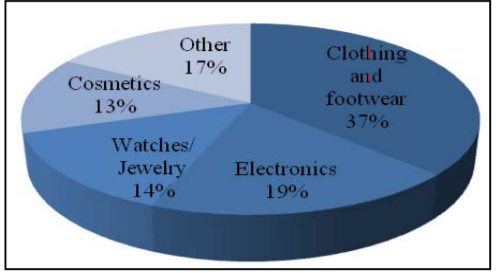
\includegraphics[width=10cm, height=7cm]{"figures/eigth.png"}
			\caption{Categorii de produse cumparate din strainatate}\label{fig:eigth}
		\end{figure}
	
	\subsection {Cercetarea B}
	\qquad Studiul de caz B este scris in 2013 si publicat in "Procedia Economics and Finance" de trei autori: Georgiana Bighiu, Adriana Manolica*, Cristina Teodora Roman. Prin aceasta lucrare se doreste a se afla daca CBD ( tulburarea de cumparare compulsiva ) se regaseste in randul studentilor din Romania care cumpara online. CBD este definita in articol drept acel „tip de comportament al consumatorului care este inadecvat, de obicei excesiv și clar perturbator pentru viața indivizilor care par impulsivi să consume”.\footnote{Bighiu Georgiana, Manolica Adriana, Roman Teodora Cristina, "Compulsive buying behavior on the internet", 2015, www.sciencedirect.com} In continuarea articolului  este specificata si explicata clar diferenta dintre achiziitle compulsive si impulsive: cumpararea compulsiva fiind atunci cand dorinta de cumparare vine din interior, poate chiar o anxietate interioara care se calmeaza prin procesul de cumparare pe cand cumpararea impulsiva este determinata de factori exteriori.
	
	\quad Studiul vizează identificarea  populației de studenți români care suferă într-un anumit grad de CBD în comportamentul lor de cumpărături online și care sunt factorii care îl favorizează. De asemenea, se sustine ideea ca stiind ce îi determină pe consumatori să cumpere fără să aibă un procesul decizional prelungit este util în proiectarea promoțiilor pentru site-urile online care vând, de exemplu, cupoanele.  
	
	\quad Obiectivul principal al studiului este de a analiza comportamentul cumpărăturilor online și de a construi un profil al studentului român ca cumpărător online compulsiv / non-compulsiv.
	
	\quad Metoda de culegere a datelor in cazul acestui studiu este tot chestionarul. Autorii au "imprumutat" adaptat si tradus in romana un chestionar de la o cercetare in italiana privind acelasi subiect. La sfarsitul colectarii de informatii s-au obtinut 100 chestionare valide de la studentii facultatii De Economie si Administrarea Afacerilor. 
	
	\qquad In urma rezultatelor obtinute s-au remarcat urmatoarele informatii: 
		\begin{itemize}
	\item dintre respondenti 81\% erau studenti de la licenta iar 19\% de la master. 
	\item Studentul FEAA folosește internetul de aproximativ 8 ani, iar in ceea ce privește obiceiurile sale de cumpărare online, cumpără online 2 produse pe lună și 19 produse pe an, în medie. In ciuda dezvoltarii metodelor de plata, studentii prefera plata traditionala in cash a produselor/serviciilor achizitionate.
	 \item În ceea ce privește articolele cele mai achiziționate online, cele mai des alese au fost articolele de îmbrăcăminte (alese de 57 de respondenți), rezultat care poate fi explicat prin faptul că două treimi dintre respondenți au fost femei, electronice sau articole de uz casnic (60/100) , bilete (autobuz, tren, avion; 49/100)
	\item Un procent de 13\% dintre respondenți s-a dovedit a avea un scor în concordanță cu tulburarea de cumpărare compulsivă. Dintre aceștia, 84,6\% erau femei, iar restul de 15,4\% bărbați confirmând rezultatele cercetării Guerreschi (2012) că majoritatea cumpărătorilor compulsivi sunt femei.
\end{itemize}
		\qquad In concluzie, profilul consumatorului compulsiv online este similar cu cel găsit în literatura scrisă despre această dependență și care confirmă studiile anterioare. Shopaholic este femeia (84,6\% dintre studenții cu CBD) cu o vârstă medie de 20 de ani, când apar de obicei primele semne ale patologiei.
		
		\quad Pe de altă parte, studentul „obișnuit” este încă blocat în modul tradițional de cumpărare demonstrând neîncredere în metodele de plată online. El / ea preferă plata la livrare care, cumva,  reduce riscul de cumpărare compulsivă, deoarece comanda poate fi anulată spre deosebire de plățile cu cardul dacă ar fi mai mult dificil. Cu toate acestea, el / ea cumpără online 19 produse pe an, indiferent dacă este vorba de haine, electronice sau bilete etc.
		\subsection{Cercetarea C}
		\qquad Ultimul studiu de caz  a fost scris tot in 2013 si publicat in revista CES Working Papers de catre Claudia Bobalca.Scopul cercetării este de a investiga percepția clienților online români cu privire la procesul de cumpărare a produselor de pe Internet. Articolul incepe cu definirea comertului electronic drept orice forma de tranzactie comerciala unde partile interactioneaza intr-o maniera electronica.\footnote{Claudia Bobalca, \textit{op.cit}, p.241}
		
		\quad Obiectivele cercetarii sunt de a afla: avantajele si dezavantajele cumparaturilor de pe internet, motivele pentru care romanii cumpara de pe Internet si motivele pentru care aleg sa cumpere de pe acelasi site.
		
		\quad In acest caz, metoda de culegere a datelor a fost interviul semi-structurat. Populatia investigata este reprezentata de clientii online din Romania care obisnuiesc sa cumpere produse de pe un site specific. 
		
		\quad Eșantionul final a fost compus din 20 de bărbați și 10 femei, deoarece cercetările de afaceri arată o rată mai mare de bărbați cumpărători online din România. Principalele produse cumpărate de participanți din magazinele online sunt: îmbrăcăminte (26 de răspunsuri), produse electronice (23 de răspunsuri), încălțăminte (17 răspunsuri), produse cosmetice (10 răspunsuri) și accesorii (7 răspunsuri).
		
		\quad Primul obiectiv a fost identificarea avantajelor și dezavantajelor cumpărăturilor online. 
		\begin{figure}[!htb]
			\centering
			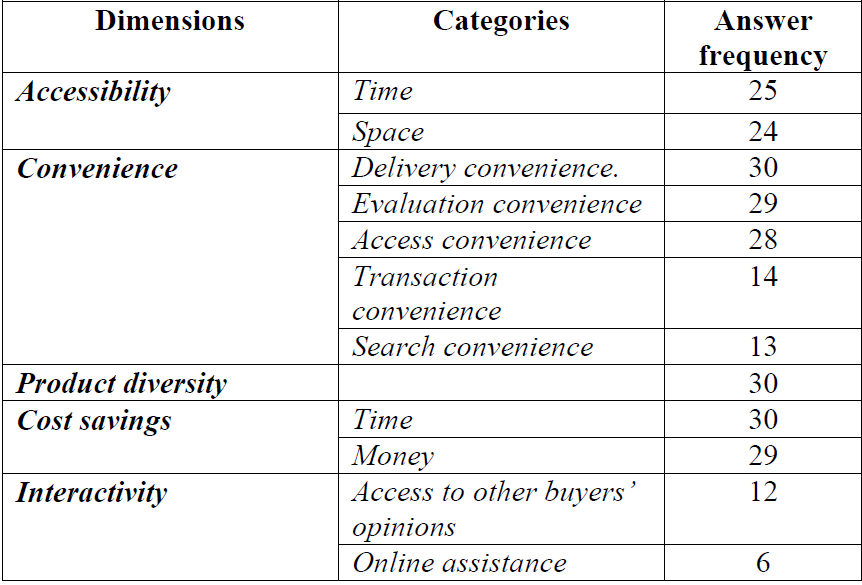
\includegraphics[width=10cm, height=7cm]{"figures/zece.png"}
			\caption{Avantajele achizitiilor online}\label{fig:zece}
		\end{figure}
	
	\begin{enumerate}[a.]
		
	\item\textbf {Accesibilitatea} este reflectată de două categorii: timp și spațiu. Cumpărarea de pe Internet elimină restricțiile de timp. De asemenea, nu există restricții de spațiu deoarece produsele pot fi cumpărate la orice oră din orice țară.
	\item\textbf{Convenienta} este formata din 5 categorii: 

	\begin{itemize}
		\item\textbf{ Acces comoditate.} Majoritatea respondenților consideră că a cumpăra de pe Internet înseamnă că nu mai trebuie să mergi într-un magazin,iar astfel poți evita locurile aglomerate.
		\item\textbf{Comoditate de căutare.} O treime dintre respondenți consideră că Internetul oferă posibilități mai bune de căutare a produselor decât magazinele tradiționale.
		\item\textbf{Confortul evaluării.} Aproape toți respondenții consideră că cumpărarea online facilitează o selecție foarte bună a produselor și produse și / sau prețuri mai eficiente și detaliate comparații. De asemenea, confortul evaluării include mai mult timp pentru respondenți să gândească, să evalueze.
		\item\textbf{Comoditatea tranzacției.} Aproximativ jumătate dintre respondenți consideră că un alt avantaj este comoditatea tranzacției: de asemenea, apreciază posibilitățile de plată.	
		\item\textbf{Confort de livrare.} Toți respondenții consideră că livrarea la domiciliu este foarte importantă si menționează si posibilitatea de a returna un produs.
	\end{itemize}
		\item\textbf{Diversitatea produselor} Toți respondenții apreciază că magazinele online oferă o mare diversitate de produse, mult mai mare uneori decât magazinele tradiționale.
		\item\textbf{Reducerea costurilor} este formata două categorii pentru dimensiunea de economisire a costurilor
	\begin{itemize}
		\item\textbf{Economisire de timp.} Toți respondenții consideră acest avantaj important.
		\item\textbf{Economie de bani.} Aproape toți respondenții menționează prețuri mai bune pentru produsele online, multe oferte speciale disponibile în mediul online și costul de livrare gratuit sau mic.
	\end{itemize}
	\item\textbf{Interactivitate} cuprinde doua categorii:
	\begin{itemize}
		\item\textbf {Acces la opiniile altor cumpărători.} Unii respondenti au spus că cumpărarea online permite clienților să acceseze feedback-ul de la alte persoane care au cumpărat de pe același site web sau din aceleași produse
		\item\textbf{Asistență online.} Unii respondenți consideră că asistența online este un avantaj.
	\end{itemize}
	\end{enumerate}
		\begin{figure}[!htb]
		\centering
		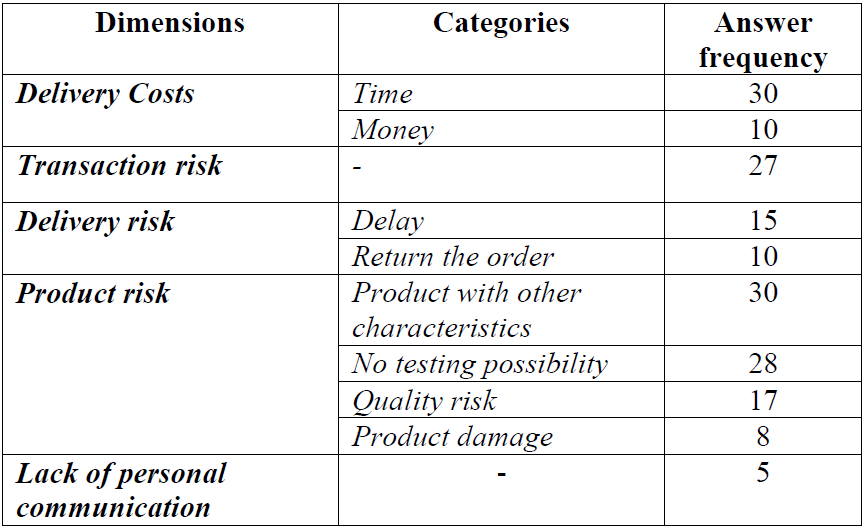
\includegraphics[width=10cm, height=7cm]{"figures/noua.png"}
		\caption{Dezavantajele achizitiilor online}\label{fig:zece}
	\end{figure}
	\begin{enumerate}[a.]
		\item \textbf {Costuri de livrare} se impart in 2 categorii:
	\begin{itemize}
		\item\textbf{Banii} O treime dintre respondenți consideră că plata costului de livrare este un inconvenient și că toate site-urile web ar trebui să aibă taxe de livrare gratuite.
		\item\textbf{Timp.} Toți respondenții au fost de acord că a cumpăra de pe Internet înseamnă a nu primi produsul pe care l-ați cumpărat la timp în aceeași zi.
	\end{itemize}
	\item\textbf{Riscul tranzacției.} În ceea ce privește riscul tranzacției, 27 de respondenți consideră că metodele de plată nesigure reprezintă o mare problemă în România.
	\item\textbf {Riscul de livrare}
		Jumătate dintre respondenți menționează ca posibile dezavantaje în ceea ce privește livrarea faptul că produsele pot îmbogăți destinația cu mare întârziere.
	\item\textbf{Riscuri privind produsele} se impart in 4 categorii:
	\begin{itemize}
	\item \textbf{Daune ale produselor.} Câțiva respondenți menționează ca dezavantaj riscul ca produsul să fie deteriorat în timpul livrării.
	\item\textbf{Produs cu alte caracteristici.} Riscul ca produsul să nu fie același cu cel comandat de un cumpărător este o mare problemă pentru toți participanții.
	\item\textbf{Risc de calitate.} Mai mult de jumătate dintre respondenți consideră că riscul de calitate este o problema importanta în comerțul electronic.
	\item\textbf{Nicio posibilitate de testare.} Faptul că produsele nu pot fi văzute, atinse sau testate înainte de cumpărături este, de asemenea, un dezavantaj menționat de participanți.
	\end{itemize}
	\item\textbf{Lipsa comunicării personale.}
		Cumpărăturile online se caracterizează printr-o lipsă puternică de comunicare personală.
		
		\quad In cadrul ultimelor doua obiective au reiesit ca cele mai importante motive pentru care participanții folosesc pentru a cumpăra din magazinele online sunt: accesibilitatea spațiului, comoditatea accesului, confortul evaluării, comoditatea livrării, economisirea timpului și economisirea banilor; iar motivațiile pentru repetarea achiziției de pe același site web sunt: calitatea produselor, diversitatea produselor, livrare rapidă, ușor de utilizat, recomandări, oferte bune, siguranță, reputație și interactivitate.
	\end{enumerate}
		
		\quad Aceste cercetari au avut fiecare o perspectiva unica deoarece cercetarea A, fiind un articol mai recent (2016) se focuseaza pe evolutia cumparaturilor online avand in vedere perspectiva consumatorilor online din Romania asupra extinderii comertului electronic inafara granitelor; Cercetarea B, are o abordare unica asupra unui concept aplicat in contextul achizitiilor online si anume CBD (tulburarea de cumparare compulsiva) dorind sa afle daca acest comportament se intalneste si al consumatorii online;iar Cercetarea C se concentreaza pe analiza avantajelor si dezavantajelor pe care consumatorii online, tineri si educati din Romania le-au intalnit de-a lungul experientelor lor. Astfel, daca am contopi toate informatiile importante de la fiecare studiu de caz, am putea spune ca avantajele si dezavantajele detaliate in cercetarea C se regasesc si in cercetarea A chiar daca exista o diferenta de 3 ani intre articole, fapt ce demonstreaza ca principalele motive pentru care consumatorii online din Romania achizitioneaza in mediul digital s-au pastrat. De asemenea, am regasit si o contradictie intre cercetarea B si cercetarea C cu privire la genul care achizitioneaza cel mai mult online si anume prima cercetare afirmand femeia cumpara cel mai des, iar a doua cercetare spunand ca barbatii.
	
	
	
	
\section{Studiu de caz }
	\subsection{Scop si obiective}
	
	\qquad In ultimii zece ani, afacerile din Romania s-au extins din ce in ce mai mult o data cu dezvoltarea mediului online, oferind o gama mult mai larga de produse, fapt ce a oferit posibilitatea oricarui consumator de a cumpara oricand si oriunde s-ar afla, doar printr-o simpla conectare la internet. Astfel, magazinele online au devenit foarte accesibile pentru populatia tanara si educata din Romania, nascuta dupa anii `90 si care este obisnuita cu boom-ul tehnologic. Aceasta cercetare isi propune sa realizeze profilul  acestui consumator online, tanar si educat din Romania.  Aceasta informatie poate fi de folos  firmelor prezente in mediul online care tintesc tocmai acest tip de consumator in demersul lor de a satisface nevoile si dorintele consumatorilor tintiti de a-i loializa respectiv de a creste numarul tranzactiilor online realizate de acestia. Pentru a analiza si mai eficient procesul decizional de cumparare online si comportamentul consumatorului online, ne-am propus trei obiective ale cercetarii: 
	\begin{enumerate}[(1)]
		\item Sa identificam ce determina consumatorii online sa achizitioneze si cum se informeaza.
		\item Sa identificam categoriile de produse si frecventa achizitiilor online.
		\item Sa identificam problemele aparute si comportamentul post-achizitie.
	\end{enumerate}
	\subsection{Metodologia cercetarii}
	\subsubsection{Metoda cercetarii}
	\qquad Pentru a atinge scopul cercetarii si pentru a obtine informatiile necesare unei analize cat mai complexe si cat mai detaliate cu referire la tema abordata in aceasta lucrare, am optat pentru o metoda de cercetare cantitativa in locul unei cercetari calitative.
	
	\quad Metoda cantitativa pe care am folosit-o in cercetare a fost sondajul de opinie, care este o metoda indirecta de colecatare a datelor. Ca si instrument al sondajului de opinie am folosit chestionarul.
	\subsubsection{Profilul respondentilor}
	\qquad Profilul respondenților la cercetarea primară cantitativă realzată stabilit a fost consumatori online (adică au avut cel putin 5 achizitii online in perioada februarie-aprilie 2021), din Romania, educați (adică fie absolvenți de studii superioare fie urmează studii universitare, în prezent), cu varsta cuprinsa intre 18-30 de ani. Am ales ca respondentii sa aiba un anumit statut socio-economic si un
	
	anumit interval de varsta deoarece considerăm că aceștia sunt mari utilizatori de tehnologie, sunt la curent cu utilizarea mijloacelor de plată electronice, se informează și respectiv reprezintă un segment de piașă important pentru comerțul electronic.
	\subsubsection{Instrumentul cercetarii}
		\qquad  Chestionarul (vezi Anexa 1) a fost lansat online cu ajutorul platformei Google Forms si a fost promovat  pe diverse grupuri de pe facebook si Instagram. Am ales aceasta metoda deoarece prezenta studentilor in acest tip de grupuri arata interesul lor de a fi constant informati, iar Facebook s-a dovedit, in experienta cercetatorului, a fi una dintre cele mai utilizate modalitati de furnizare a informatiilor studentilor. Astfel, orice student din Romania, care apartinea segmentului tinta, putea completa chestionarul online, iar odata completat acesta intra direct in baza de date. Aceasta tehnica este una destul de rapida deoarece chestionarul dureaza 7-8 minute maxim pentru a-l completa si nu implica costuri deoarece Google Forms este o platforma gratuita.

		\quad Chestionarul (vezi Anexa 1) a cuprins un numar de 16 intrebari obligatorii,unele intrebari fiind cu mai multi itemi de raspuns pentru a oferi posibilitatea respondenților de a alege răspunsul cel mai apropiat situației personale. Chestionarul a cuprins 13 intrebari inchise si doar doua intrebari deschise. Am optat pentru această structură a întrebărilor deoarece în cazul întrebărilor închise se răspunde rapid și ușor – aspecte care conduc la creșterea ratei de răspuns la chestionar. Întrebările deschise  ajută la culegerea de date de profunzime, extrem de relevante pentru cercetare dar intervin și două impediente, fie respondenții nu răspund deloc la ele fie dau răspunsuri extrem de lapidare care nu ajută penstru scopul cercetăroo.. Pentru a intelege mai bine structura chestionarului l-am impartit in 3 sectiuni astfel::
		\begin{enumerate}[(1)]
			\item\textbf{Intrebarile de la 1-3} (1)	Intrebarile de la 1-3 sunt intrebari filtru care stabilesc daca respondentul se in- cadreaza in profilul respondentilor stabilit in scopul pentru aceasta cercetare si anume educat (adică să aibă calitatea de student sau absolvent de studii europene), tânăr (adică cu varsta cuprinsa intre 18-30 de ani) si cu achiziții online (adică peste 5 achizitii online in perioada februarie-aprilie 2021). Chestionarul fiind realizat în limba română, implict ne-am adresat consumatorilor români. 
			\item\textbf{Intrebarile de la 4-10} reprezinta chestionarul propriu zis, care de asemenea le-am grupat in 5 grupe.
		\begin{enumerate}[(a)]
			\item Prin \textbf{intrebarile de la 4 la 7} am dorit sa aflam mai multe detalii despre procesul de cautare si analiza a informatiei pe care consumatorii o gasesc accesibila online.
			\item Prin \textbf{intrebarile 8 si 9} sa identificam ce categorii de produse cumpara cel mai des online si cat de frecvent plaseaza comenzi online.
			\item Prin\textbf{intrebarile de la 10 la 13} am vrut sa analizam problemele aparute in momentul plasarii unei comenzi si comportamentul consumatorilor online post-achizitie, avand si doua intrebari deschise \textbf {12-13} care le ofera posibilitatea respondentilor sa se exprime liber cu privire la cea mai buna si cea mai putin buna experienta a lor online.
		\end{enumerate}
		\item\textbf{Intrebarile de la 11-13}sunt cele care completeaza profilul respondentului cu caracteristici ca: gen, nivelul studiilor si numarul mediu de ore pe care il petrec online inafara cursurilor online. Am decis sa culegem aceste informatii pentru a putea apoi sa incadram respodentii intr-o anumita categorie, fapt ce ne va ajuta la analiza datelor.
		\end{enumerate}
	
		\quad Pentru a nu exista intrebari neclare, variante de raspuns irelevante sau variante de raspuns incomplete, am pretestat chestionarul inainte de lansare. Astfel, am trimis chestionarul la doi colegi-studenti, care se încadrează în profilul respondenților acestei cercetări. Ulterior, pe baza feedback-ului primit din partea celor doi respodenti au aparut mici modificari in structura chestionarului.
		
		\quad Chestionarul a fost lansat in data de 27 aprilie 2021 si a fost valabil pana in data de 4 mai 2021. In aceasta perioada au raspuns la chestionar un numar de 202 de respondenti, dintre care 106 raspunsuri valide, de la respondenti care au ales la intrebarea filtru peste 5 achizitii online in perioada data si 96 raspunsuri nevalide, de la respondenti care au ales mai putin de 5 achizitii online in periodata mentionata.
	
		
	\subsection{Analiza si intepretarea datelor}
		\qquad Datele culese din sondajul de opinie au fost culese cu ajutorul unui chestionar (vezi Anexa 1), lansat online, in perioada 27 aprilie- 4 mai 2021. Pentru lansarea chestionarului am folosit aplicatia Google Forms. Avantajul utilizarii acestei aplicatii consta in faptul ca raspunsurile primite sunt centralizate si prelucrate in mod automat. Un alt avantaj al utilizarii Google Forms ca mijloc de a distribui un sondaj consta in generarea automata de grafice pe baza raspunsurilor primite. 
		
		\qquad Asa cum am mentionat anterior, la sondajul de opinie lansat am primit un numar de 202 de raspunsuri din care 96 nu au fost valide. Practic, validitatea chestionarelor a fost dată de răspunsul pozitiv la întrebările filtru. Astfel, cei 96 de respondenți a căror chestionare completate nu au fost validate, nu s-au încadrat în publicul țintă al prezentei cercetări.  Ca urmare, marimea esantionului sondajului de opinie realizat este de 106 de respondenti. Rezultatele obtinute vor fi prezentate in continuare.
		
		\qquad Profilul respondentilor studiului de caz din intrebarile rezultate din intrebarile de identificare este prezentat in continuare:
		\begin{itemize}
			\item Din datele obtinute (vezi fig.11) putem observa ca din totalul respondentilor cei mai multi (57,5\%) petrec mai mult de 3 ore online ceea ce subliniaza ca mediul online este foarte accesibil si atragator pentru consumatorii online, 34\% sustin ca petrec cate 2-3 ore , ceea ce tot reprezinta mult avand in vedere contextul cursurilor online, iar 8,5\% dintre respondenti petrec mai putin de 2 ore, ceea ce subliniaza suprasaturatia  fata de mediul online.
			\begin{figure}[!htb]
				\centering
				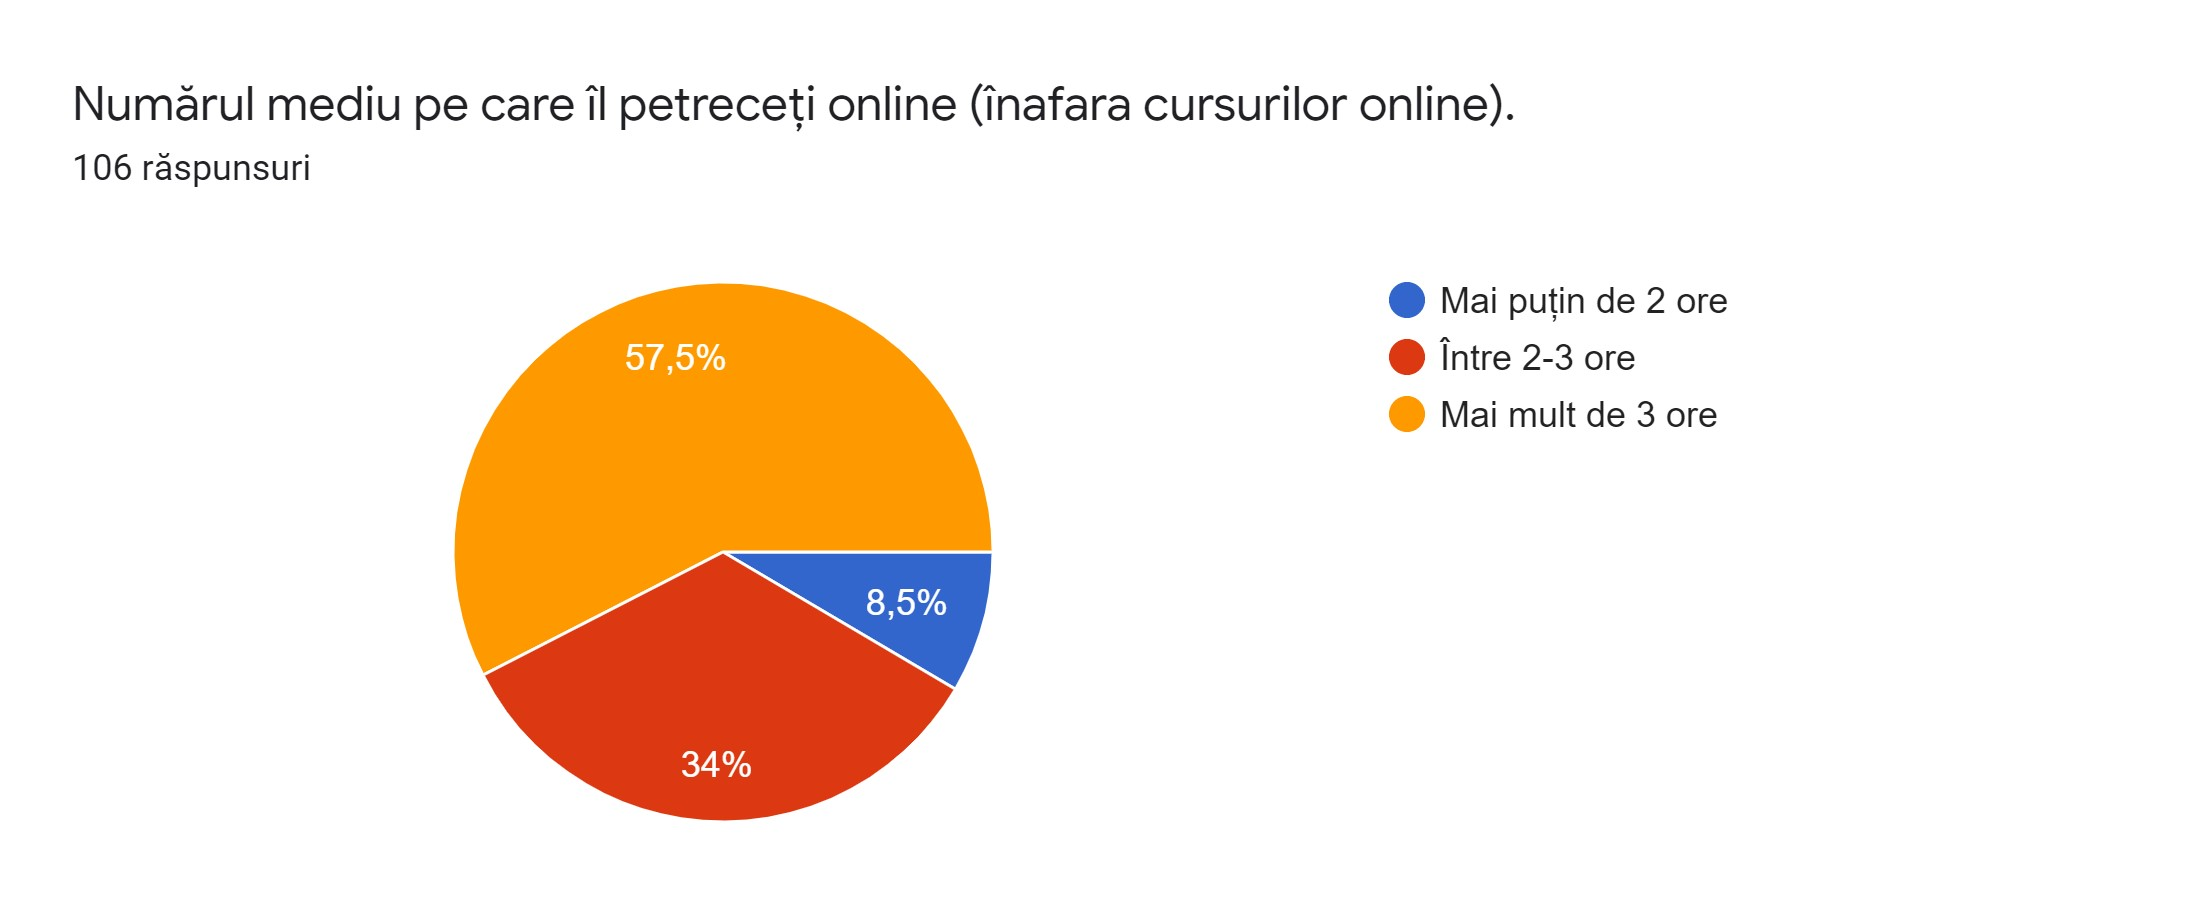
\includegraphics[width=13cm, height=6cm]{"figures/prima.jpg"}
				\caption{Figura 3.1.Repartitia respondentilor dupa numarul mediu de ore petrecut online}\label{fig:zece}
			\end{figure}
	\newpage
		\item Referitor la nivelul de studii absolvit al respondentilor (vezi fig.12), esantionul nostru este format  preponderent de absolventi de studii superioare (mai exact 61,3\%), restul fiind în prezent studenți. Mai mult, din tot eșantionul 22,6\% au studii post-universitare.
			\begin{figure}[!htb]
			\centering
			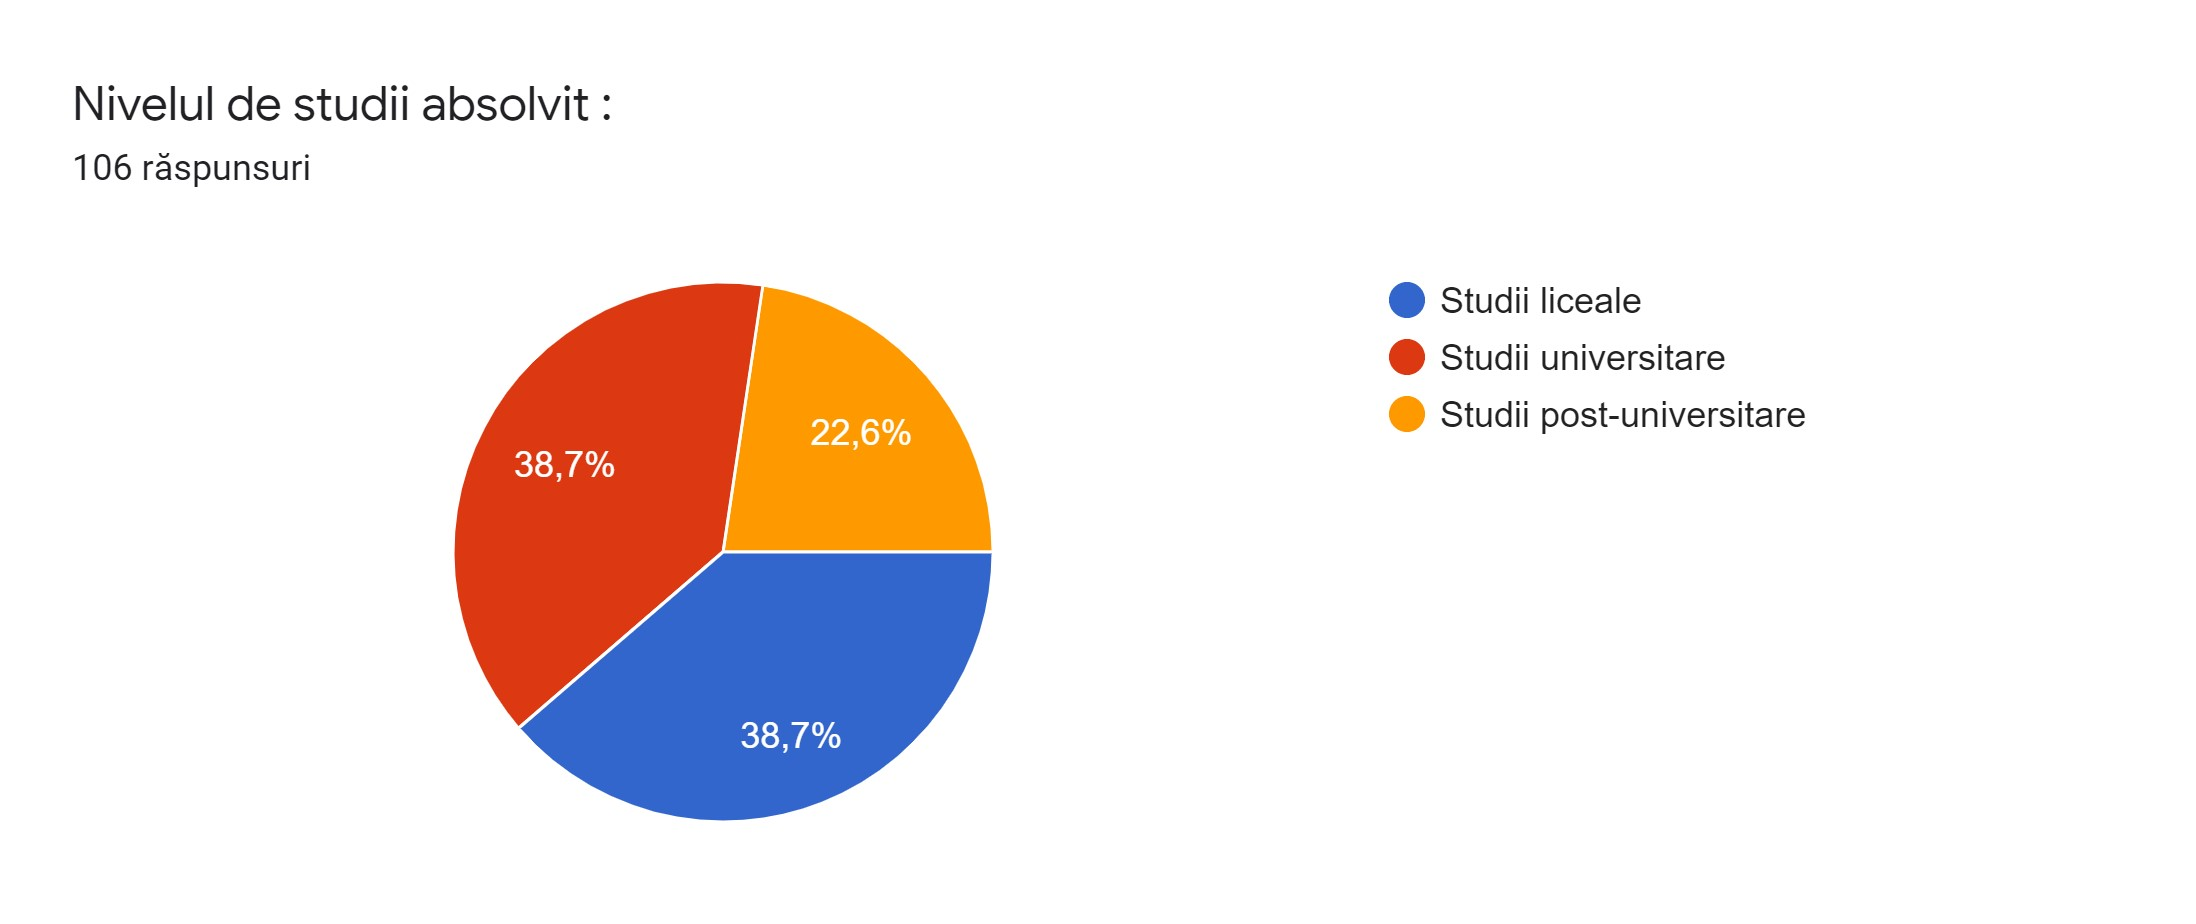
\includegraphics[width=13cm, height=6cm]{"figures/doi.jpg"}
			\caption{Figure 3.2. Repartia respondentilor dupa nivelul de studii absolvit}\label{fig:zece}
		\end{figure}
		\item Din perspectiva genului, marea majoritate a respondentilor sunt de gen feminin, cu un procent de 90,6\% care indica faptul ca femeile sunt mai empatice pentru a raspunde la chestionare online deoarece studiile analizate anterior nu au indicat nicio diferenta atat de mare intre cele doua sexe. Astfel, acest lucru nu inseamna ca barbatii achizitioneaza mai putin, deoarece numarul scazut de respondenti de gen masculin reflecta doar o limita a cercetarii noastre.
		\end{itemize}
	\qquad Pentru urmatoarea parte lucrarii, vom analiza principalele constatări ale
	eșantionarii populației, luând în considerare cele trei obiective definite anterior.
	\begin{enumerate}[(A)]
		\item Primul obiectiv al studiului nostru: sa identificam ce determina consumatorii online sa achizitioneze din mediul online si cum se informeaza.
		
		\qquad Pentru a identifica motivele pentru care consumatorii online prefera sa achizitioneze din mediul online si care este atitudinea lor fata de beneficiile achizitiilor online, am adaugat o intrebare cu 5 itemi de raspuns (Posibilitatea de a realiza comparații, Accesibilitatea 24/24, Oportunitatea de a plăti un preț mai mic, Acces la gama mai larga de produse, Abilitatea de a împărtăși experiențe pe rețelele de socializare), unde respondentii trebuiau sa masoare pe o scara de la 1 la 5 gradul de intensitate al fiecarui item in parte(vezi intrebarea 4 - Anexa 1). Raspunsurile primite sunt reprezentate mai jos(vezi tabelul 3.1). \textbf{Repartitia respondentilor dupa raspunsurile la intrebarea...}
		\newcolumntype{M}[1]{>{\centering\arraybackslash}m{#1}}
		\begin{center}
			
			\begin{tabular}{ | M{16em} | M{1.1cm}| M{1.1cm} | M{1.1cm}| M{1.1cm} | M{1.1cm} | } 
				\hline
				\centering
	
				& 1 & 2 & 3 & 4 & 5\\ 
				\hline
				Posibilitatea de a realiza comparatii & 2,8\% & 10,4\%  & 28,3\% & 22,7\% &35,8\%   \\ 
				\hline
				Accesibilitatea 
				24/24  & 2,8\%  & 0,9\%  & 19,8\% &19,8\%  & 55,7\% \\ 
				\hline
				Oportunitatea de a plăti un preț mai mic & 0,9\% & 6,5\%  &20,8\%  &20,8\% & 51\%  \\ 
				\hline
				Acces la o gamă mai largă de produse &0\%  &4,7\%  & 16\%  & 23,6\% & 55,7\% \\ 
				\hline
				Abilitatea de a împărtăși experiența online &33\%  & 13,2\%  &22,7\%  &16\% &14,1\% \\
				\hline
			\end{tabular}
			\newline
		\end{center}
	
	\qquad Asadar, prin raspunsurile obtinute la aceasta intrebare( vezi Tabelul 3.1.) putem deduce urmatoarele:
	\begin{itemize}
		\item \textit{accesibilitatea 24/24} si \textit{accesul la o gama mai larga de produse}  (ambele detinand un procent de 55,70\%) sunt principalele beneficii pentru care consumatorii online obisnuiesc sa achizitioneze din mediul online , avantaje ce deosebesc magazinele virtuale de cele traditionale.
		\item Urmatorul beneficiu care a fost ales de catre 51\% dintre respondenti, se refera la \textit{oportunitatea de a plati un pret mai mic} deoarece magazinele online nu au anumite costuri precum chiria spatiului si a utilitatilor, fapt ce reprezinta un mare plus pentru cumparatori.
		\item  Pe de alta parte, cel mai putin important beneficiu al comertului electronic ales de respondenti a fost \textit{abilitatea de a impartasi experienta online}, ceea ce indica faptul ca impartasirea experientei personale nu are loc exclusiv in mediul online.
	\end{itemize}
	
	\qquad Pentru a identifica sursele de informare pe care se bazeaza consumatorii online in momentul in care vor sa realizeze achizitii online, am introdus 4 itemi ( Experienta personala, Review-urile de pe site, Opiniile celor apropiati, Informatia oferita de motoarele de cautare), prin care respondentii au putut acorda o nota de la 1 la 5 (in ordine crescatoarea a intensitatii pe care o simte fiecare subiect asupra itemului respectiv)(vezi Intrebarea 5 Anexa 1). Raspunsurile sunt prezentate mai jos(Vezi tabelul 3.2))
	
	\newcolumntype{M}[1]{>{\centering\arraybackslash}m{#1}}
	\begin{center}
		\begin{tabular}{ | M{14em} | M{1.1cm}| M{1.1cm} | M{1.1cm}| M{1.1cm} | M{1.1cm} |} 
			\hline
			& 1 & 2 & 3 & 4 & 5\\ 
			\hline
			Experienta personala  & 2,8\% & 1,9\% &10,4\%  & 28,3\% & 56,6\% \\ 
			\hline
			Review-urile de pe site  &0,9\%  &5,7\%   &27,4\%  &39,6\%  &26,4\%\\ 
			\hline
			Opiniile celor apropiati & 3,7\% & 3,7\%  & 29,2\%  & 35,8\% & 26,4\% \\ 
			\hline
			Informatia oferita de motoarele de cautare & 9,4\% &10,4\%  &34,9\%  &34,9\% & 10,4\% \\ 
			\hline
		\end{tabular}
		\newline
	\end{center}
	\qquad Conform datelor culese, in momentul achizitiei unui produs online, consumatorii se bazeaza cel mai mult pe\textit{ experienta personala} din trecut, detinand cel mai mare procent (84,9\%),urmand apoi cu un procent de 66\% \textit{review-urile de pe site}. Acest fapt denota un aspect neasteptat si anume o incredere mai mare asupra review-urilor online decat in opiniile celor apropiati. Cel mai mic procent (45,3\%) l-a obtinut informatia oferita de motoarele de cautare,acest lucru putand fi datorat fie volumului mare de date disponibile online, fie gradului  scazut de acuratete a informatiei prezente pe internet.
	
	\qquad Pentru a identifica elementele care conteaza cel mai mult pentru consumator atunci cand ia decizia de a alege un magazin online in detrimentul altuia, am introdus o intrebare cu 5 itemi(Brand-ul produsului, Usurinta utilizarii site-ului, Politica de Return, Diversitatea gamei de produse, Posibilitatea de a urmari comanda realizata), prin care respondentii au putut acorda o nota de la 1-5 in ordinea crescatoare a intensitatii pe care o simte fiecare subiect asupra item-ului respectiv(vezi intrebarea 5 Anexa 1). Raspunsurile sunt prezentate mai jos.(vezi tabelul 3.3)
	\newcolumntype{M}[1]{>{\centering\arraybackslash}m{#1}}
		\begin{center}
		\begin{tabular}{ | M{15em} | M{1.1cm}| M{1.1cm} | M{1.1cm}| M{1.1cm} | M{1.1cm} |} 
			\hline
			& 1 & 2 & 3 & 4 & 5\\ 
			\hline
			 Brand-ul produsului &1,9\%  &10,4\%  & 41,5\%  &21,7\% &24,5\% \\ 
			\hline
		     Usurinta utilizarii site-ului& 3,8\% & 3,8\%   &17\%  &37,7\%  &37,7\% \\ 
			\hline
			Politica de Return & 5,7\%  &9,4\%  &18,9\%  &33\% &33\% \\ 
			\hline
			Diversitatea gamei de produse & 0,9\%  &2,8\%  &13,2\%  &33\% &50\% \\ 
			\hline
			Posibilitatea de a urmari comanda realizata & 2,8\%  & 6,6\%  &18,9\%  &32,0\% &39,6\% \\
			\hline
		\end{tabular}
		\newline
		\end{center}
		\qquad Potrivit raspunsurilor primite, am obtinut urmatoarele rezultate:
		\begin{itemize}
			\item Jumatate din totalul de respondenti au oferit grad maxim item-ului privind \textit{diversitatea gamei de produse}, acesta avand si cel mai mare procent (83\%), rezultat ce denota atractia consumatorului fata de un magazin mixt  in locul unuia specializat pe o singura gama de produse. Acest lucru se datoreaza faptului ca procesul de achizitie a consumatorului se simplifica, acesta avand posibilitatea de a cumpara mai multe produse dintr-un singur loc.
			\item Pe urmatorul loc, cu procentul de 75,4\%, este \textit{usurinta utilizarii site-ului} element ce determina importanta nivelului de accesibilitate al paginii web pentru consumatorii care obisnuiesc sa achizitioneze online.
			\item Un alt aspect interesant este faptul ca \textit{Politica de return }are un scor mediu (66\%), fapt ce pune la indoiala informatiile pe care le au consumatorii cu privire la drepturile lor privind returnarea bunurilor achizitionate. 
			\item De asemenea, contrar asteptarilor, elementul cu cele mai putine voturi il reprezinta \textit{brand-ul produsului} avand un procent de doar 46,2\%, care indica faptul ca, in prezent, consumatorii nu mai pun cel mai mare accent pe notorietatea  magazinului de la care cumpara, ci se focuseaza pe alte elemente in procesul  decizional, precum cele amintite anterior.
		\end{itemize}
		
		\quad Referitor la nivelul de documentare a consumatorilor inaintea plasarii unei comenzi online, am introdus o intrebare cu un singur item prin care respondentii au putut acorda o nota de la 1 la 5 in ordinea crescatoare a intensitatii cu care se informeaza.
		
		\begin{figure}[!htb]
			\centering
			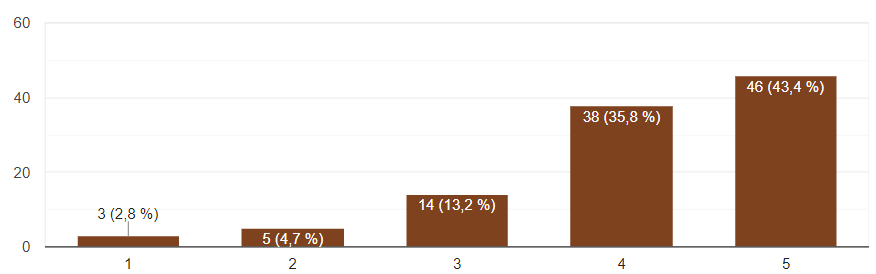
\includegraphics[width=14cm, height=5cm]{"figures/trei.png"}
			\caption{Figure 3.3 Repartizarea respondentilor dupa nivelul de documentare a respondentilor inainte de a comanda online}\label{fig:unuspre}
		\end{figure}
	
	 	\qquad Asadar, prin raspunsurile oferite se observa ca respondentii au un nivel crescut de maturitate, alegand sa se informeze riguros inainte de a alege sa cumpere un produs, deoarece  35,8\% au ales ca se informeaza mult, iar 43,4\%, aproape jumatate, au ales chiar grad maxim de informare. Acest fapt este subliniat si de faptul ca doar 2,8\% din respondenti au ales cea mai mica nota (1) care inseamna informare deloc.

	 	
		\item Al doilea obiectiv al studiului nostru : sa identificam categoriile de produse si frecventa achizitiilor online.
		
		\quad Pentru a identifica categoriile de produse cele mai achizitionate in mediul online, am propus acestora sa raspunda care e categoria de produse pe care o cumpara cel mai des online.(vezi intrebarea 7 Anexa 1).
		
		\begin{figure}[!htb]
			\centering
			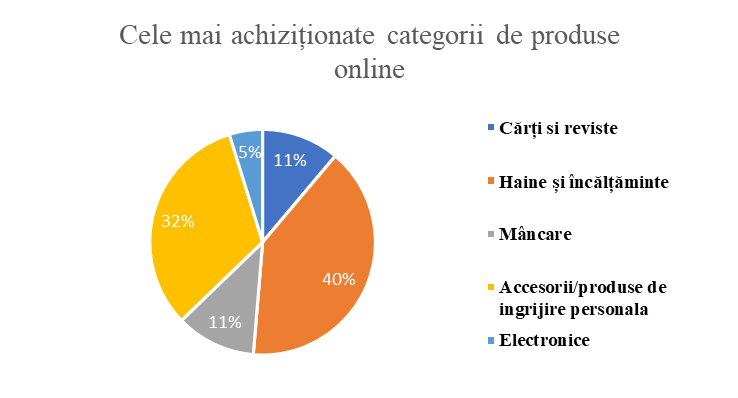
\includegraphics[width=13cm, height=6cm]{"figures/patru.png"}
		\end{figure}
	
		\quad Cei mai multi dintre respondenti ( vezi figura 3.4) au raspuns ca\textit{ hainele si incaltamintea} reprezinta cea mai frecventa categorie de produse achizitionata. Pe locul doi se afla \textit{accesoriile/ produsele de ingrijire personala}, iar pe trei,\textit{ cartile si revistele} aflandu-se la egalitate cu \textit{mancarea}. Aceste categorii de produse au fost bunurile care au fost cele mai importante pentru consumatorii online, tineri si educati din Romania in perioada februarie-aprilie 2021.
	
		\qquad Pentru a cunoaste frecventa  cu care consumatorii achizitioneaza, in mediul  online, am propus acestora sa raspunda cat de frecvent obisnuiesc ei sa achizitioneze produse sau servicii cu ajutorul internetului fie de pe laptop/telefon sau tableta(vezi intrebarea 8, Anexa 1)
	
		\begin{figure}[!htb]
			\centering
			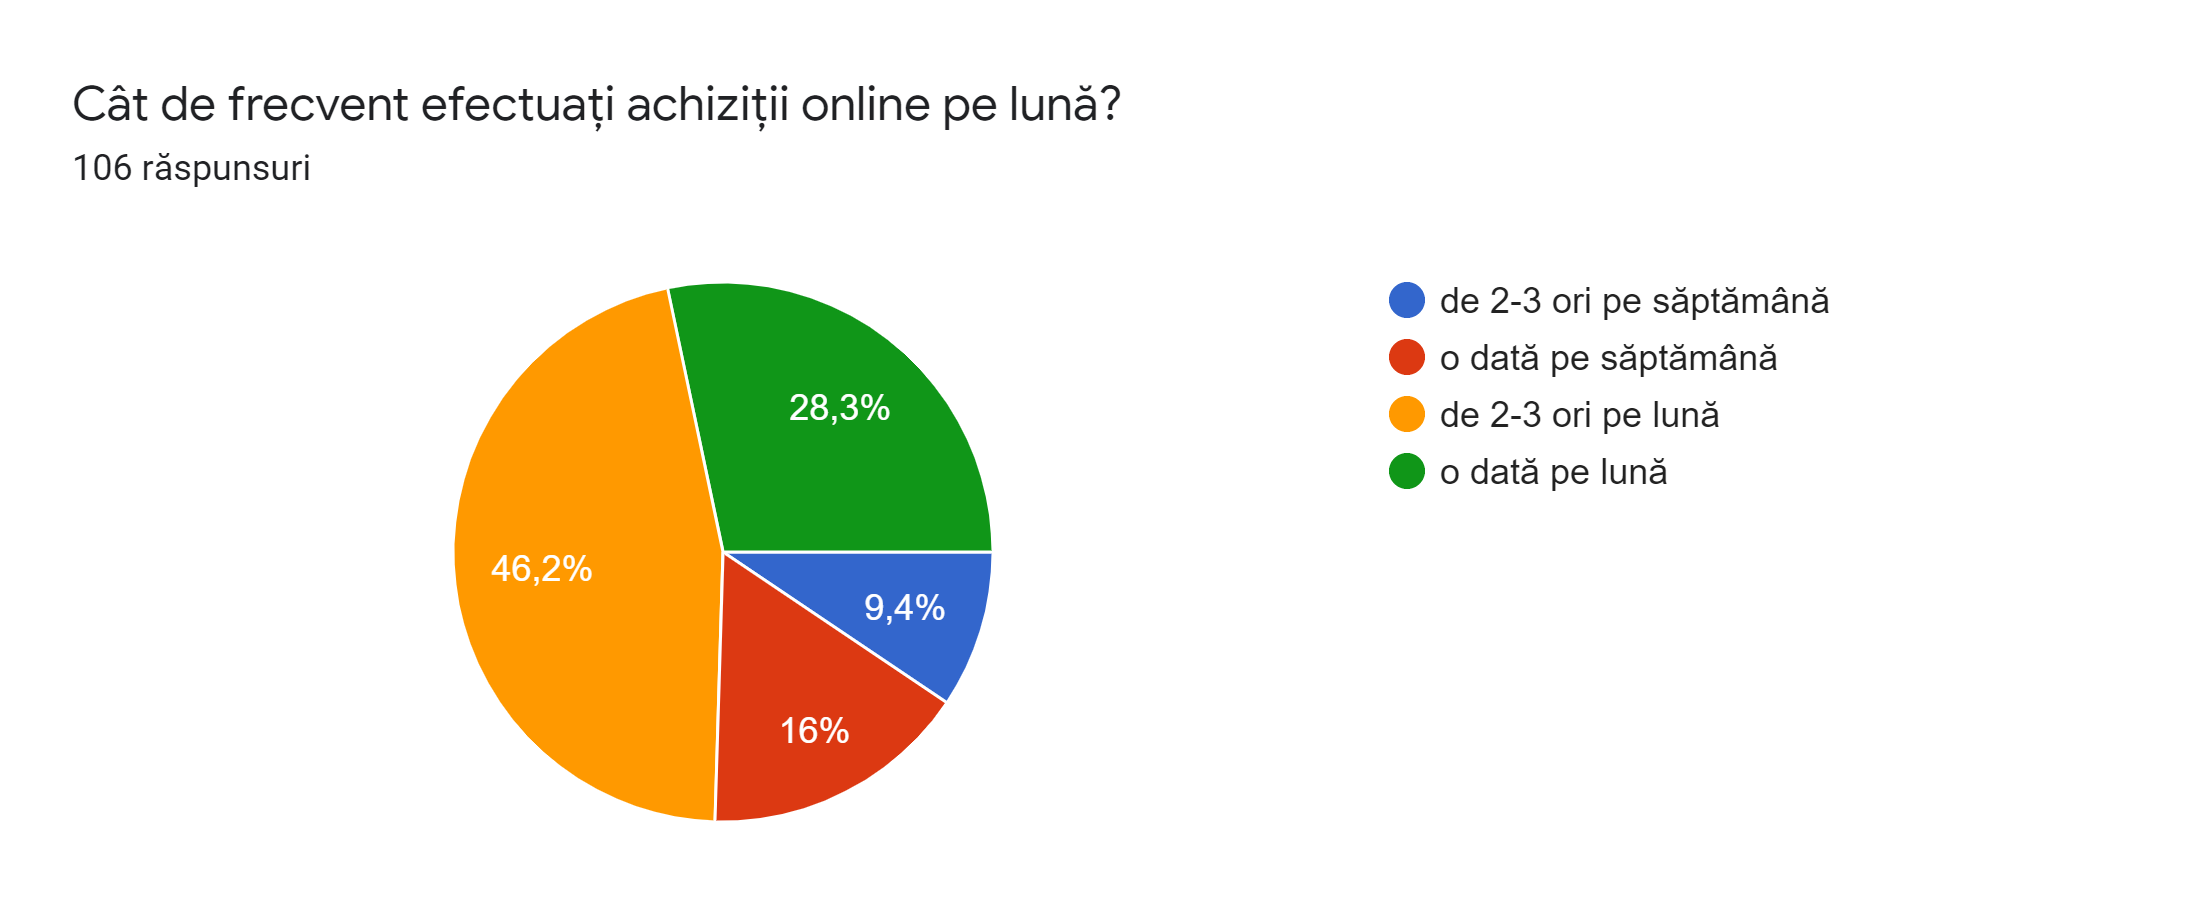
\includegraphics[width=16cm, height=7cm]{"figures/cinci.png"}
		\end{figure}

		\qquad Conform raspunsurilor culese,(vezi Figura 3.5) cei mai multi respondenti (46,2\%) au spus ca achizitioneaza de \textit{2-3 ori pe luna}, fapt ce se incadreaza ca o medie intre des si rar, iar cei mai putini respondenti (9,4\%) au spus ca achizitioneaza de \textit{2-3 ori pe saptamana}.
	
		\item Al treilea obiectiv al studiului nostru: Sa identificam problemele aparute si comportamentul post-achizitie.
\end{enumerate}		

		\quad Pentru a afla ce tip de probleme au intampinat atunci cand au achizitionat un produs online, am adaugat o intrebare cu 5 itemi (Timpul de livrare nu a fost respectat, Produsul a ajuns cu defecte, Au fost costuri mari cu livrarea, Calitate inferioara, Returnarea produsului a fost dificila)prin care respondentii au putut acorda o nota de la 1-5 in ordinea crescatoare a intensitatii pe care o simte fiecare subiect asupra item-ului respectiv(vezi intrebarea 9, Anexa 1). Raspunsurile sunt prezentate mai jos(vezi tabelul 3.4).
	\newline
		
		\newcolumntype{M}[1]{>{\centering\arraybackslash}m{#1}}
		\begin{center}
			\begin{tabular}{ | M{16em} | M{1.1cm}| M{1.1cm} | M{1.1cm}| M{1.1cm} | M{1.1cm} |} 
				\hline
				& 1 & 2 & 3 & 4 & 5\\ 
				\hline
				Timpul de livrare nu a fost respectat  &8,5\%  &37,7\%  &27,4\%  &18,9\% &7,5\% \\ 
				\hline
				Produsul a ajuns cu defecte &34\%  &44,3\%   &17\%  &4,7\%  &0\%\\ 
				\hline
				Au fost costuri mari cu livrarea &13,2\%  & 26,4\%  &29,2\%  &18,9\% &12,3\% \\ 
				\hline
				Calitate inferioara &18,9\%  &41,5\%  & 24,5\%  &12,3\%  &2,8\% \\ 
				\hline
				Returnarea produsului a fost dificila & 32,6\%  & 27,4\%  & 18\% & 9,4\% &5,7\% \\
				\hline
			\end{tabular}
	\newline
		\end{center}
	\qquad\space\space Potrivit datelor culese(vezi tabel 3.4), consumatorii nu au prea intalnit acest tip de probleme atunci cand au plasat o comanda online, fapt dovedit de notele mici acordate problemelor din figura de mai sus. Cea mai intalnita, dar care tot detine un scor nu foarte mare (31,2\%) este \textit{costuri mari cu livrarea}, urmand pe locul doi, cu un procent de 26,4\%, \textit{timpul de livrare care nu a fost respectat} fapt ce subliniaza importanta calitatii livrarii bunurilor in procesul de achizitie online. Problema intalnita cel mai putin a fost \textit{Produsul a ajuns cu defecte} avand un procent de aproape 5\%.
	
	\quad Pentru a identifica cum reactioneaza consumatorii  online atunci cand intalnesc o problema cu produsul livrat de la un magazin online, am intrebat cum au actionat ei dupa ce au constat ca bunul primit in urma comenzii, nu este conform cerintelor lor. Raspunsurile sunt prezentate mai jos(vezi figura 3.6).
	
	
	\begin{figure}[!htb]
		\centering
		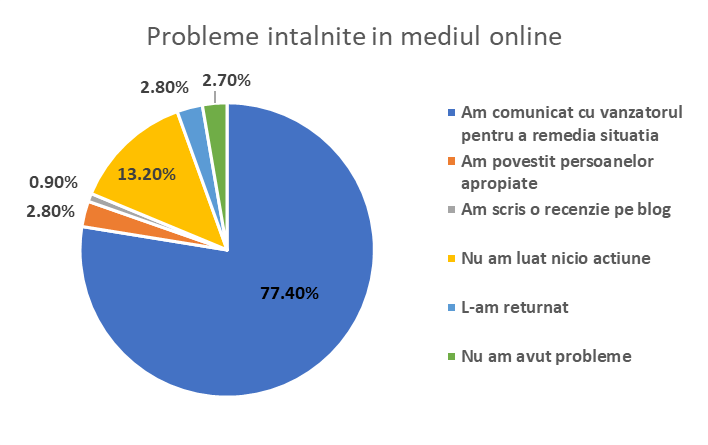
\includegraphics[width=12cm, height=7cm]{"figures/sapte.png"}
	\end{figure}

	\quad Conform raspunsurilor obtinute, am constat ca cei mai multi respondenti, anume un procent de 77,4\% din total au raspuns ca ei comunica problema intalnita vanzatorului/ magazinului de la care a achizitionat bunul pentru a putea remedia si rezolva situatia creata, fapt ce subliniaza inca o data seriozitatea si increderea de care da dovada consumatorul fata de achizitiile din mediul online. Acest lucru evidentiaza profilul stabilit al participantilor, la acest studiu, inca de la inceputul cercetarii. Din pacate, au existat si persoane (13,20\%) care au ales sa nu ia nicio actiune cu privire la bunul achizitionat si neconform cerintelor si asteparilor lor. Au existat si cateva pareri, in minoritate, care au ales sa actioneze diferit si unic precum: impartasirea experientei celor apropiati(2,8\%), returnarea produsului (2,8\%) si scrierea experientei pe un blog (0,9\%).
	
	\quad In ultima parte a analizei datelor culese doresc sa integrez intrebarile deschise de la finalul chestionarului (vezi intrebarea 12 si 13, Anexa 1) alaturi de celelalte intrebari pentru a crea un profil al respondentilor bazat pe cele 3 categorii de varsta (18-21, 22-24, 25-30) si pentru a putea identifica diferentele ce pot aparea intre segmentele de clienti, in functie de categoria de varsta. 
	
	\quad In cadrul intrebarile deschise, privind experientele consumatorilor, am dorit sa vedem ce considera  el ca fiind cea mai buna experienta in mediul online si problemele care l-au determinat sa vada o alta experienta, drept cea mai putin buna.
	
	\quad Din cauza ca predomina  respondentii de gen feminin  cu peste 90\% din esantion, voi analiza in continuare raspunsurile primite de la ele.
	
	\quad Faptul ca procentul raspunsurilor feminine excede procentul raspunsurilor masculine poate indica faptul ca femeile sunt mai empatice la raspunderea de chestionare online decat barbatii sau poate fi datorat implicarii unui numar restrans de respondenti de gen masculin in completarea chestionarului.

	\quad Din procentul de 90,6\% din totalul persoanelor care au raspuns la chestionar, 33\% dintre respondentii de gen feminin au varsta cuprinsa intre 18-21 de ani( abia au terminat studiile liceale sau sunt studente la o facultate), 29\% au varsta cuprinsa intre 22-24 ( sunt absolvente de licenta sau studente la master), 38\% au varsta cuprinsa intre 25-30 de ani (fie sunt absolvente de studii superioare sau studente la doctorat)(vezi figura 3.7).
		\begin{figure}[!htb]
		\centering
		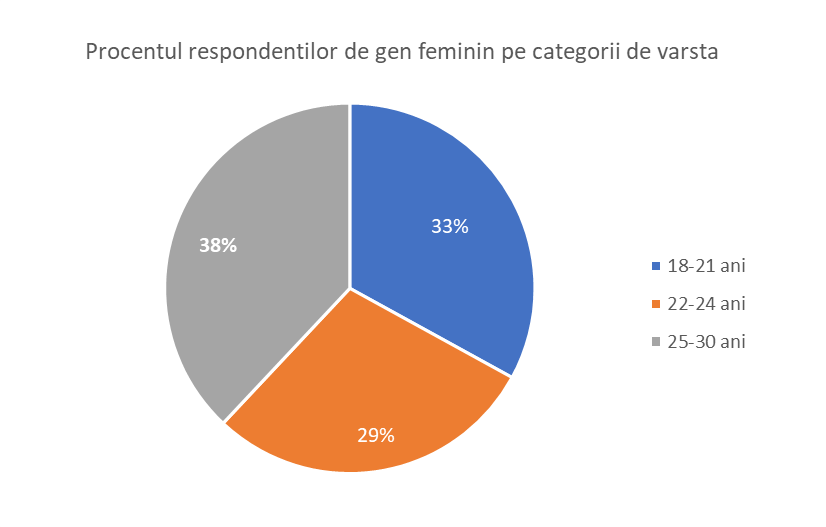
\includegraphics[width=12cm, height=6cm]{"figures/ana.png"}
	\end{figure}
	
\newpage	
	\begin{itemize}
		\item \textbf{Prima categorie de varsta (18-21 ani)} reprezinta 33\% din totalul de respondenti de gen feminin. In  urma analizei asupra datelor oferite, am extras informatiile relevante pentru a putea sublinia caracteristicile acestei categorii. 
		
		\quad Primul lucru pe care l-am sesizat a fost faptul ca 57\% dintre respondentii acestei categorii petrec mai mult de 3 ore online, inafara cursurilor de la facultate, insa frecventa cu care comanda online este redusa, procentul de  37\% spunand ca plaseaza comenzi o data pe luna . Acest lucru releva un paradox si anume, daca o persoana petrece mult timp in mediul online nu inseamna ca isi face cumparaturile tot in acest mediu.
		
		\quad Urmatorul lucru pe care l-am identificat a fost faptul ca\textit{ hainele si incaltamintea} reprezinta cea mai frecventa categorie de produse achizitionata online (50\% au ales aceasta categorie),  fapt ce releva increderea pe care o au acesti consumatori tineri in aceste magazine. Acest lucru este subliniat si de procentul ridicat de 68,8\% in care acestia au raspuns ca atunci cand apar eventuale erori cu comanda sau produsul achizitionat au siguranta ca pot comunica cu producatorul pentru a remedia situatia ulterior. 
		
		\quad Pentru a analiza raspunsurile oferite de respondenti la intrebarile deschise am decis sa grupam experientele impartasite pentru a le evidentia pe cele care s-au afirmat cel mai mult:
		\begin{itemize}
			\item In cazul intrebarii deschise referitoare la cea mai buna experienta pe care au avut-o pana acum, consumatorii au subliniat in mare parte avantajele pe care magazinele online le ofera cumparatorilor si care conteaza cel mai mult pentru ei. Dintre acestea enumeram: rapiditatea livrarii produsului intr-un timp cat mai scurt, fiind cel mai des mentionat element, urmand apoi disponibilitatea producatorului de a raspunde si remedia eventuale erori si apoi posibilitatea de a urmari produsul achizitionat in timp real.
			\item 	In cadrul intrebarii referitoare la experienta mai putin buna s-au accentuat problemele pe care consumatorii le-au intalnit. Dintre acestea, cel mai mult s-au mentionat timpul de livrare care nu a fost respectat si neconcordanta dintre calitatile promise in mediul online fata de cele primite la momentul livarii produsului. 
		\end{itemize}
		\item \textbf{A doua categorie de varsta (22-24 ani)} este reprezentata de 29\% din totalul de respondenti de gen feminin. In aceasta categorie s-au sesizat mici diferente, fata de cea analizata anterior pe care le voi prezenta in randurile urmatoare.
		
		\quad Prima diferenta pe care am sesizat-o la femeile e-consumator, cu varsta cuprinsa intre 22-24, este ideea ca in ciuda faptului ca petrec tot la fel de mult timp online ca si generatia anterioara, procentul de achizitii online cel mai mare (60\%) este la varianta cu 2-3 achizitii pe luna. Acest fapt ne indica ca femeile sunt mult mai atente cu programul lor si ca incearca sa-si organizeze cat mai eficient activitatile ce necesitau ore inainte in magazinele fizice, dar posibile doar cu un click in mediul online.
		
		\quad Urmatoarea diferenta pe care am observat-o a fost la categoriile de produse achizitionate cel mai des online. Fata de generatia anterioara, respondentii de gen feminin din aceasta categorie au un procent mai scazut (42,9\%) la categoria de \textit{haine si incaltaminte}, urmat de \textit{accesorii si produse de ingrijire} cu un procent de 35,8\%. Acest lucru dezvaluie tendinta fetelor de a pune mult mai mare accent pe ingrijirea personala cu inaintarea in varsta. 
		
		\quad La intrebarile deschise aflate la finalul chestionarului, fetele au mentionat aproximativ aceleasi elemente care s-au amintit, referitoare la experientele pozitive si negative pe care le-au avut, in schimb, s-au sesizat cateva elemente de noutate precum:
		\begin{itemize}
			\item In cadrul celei mai bune experiente s-a adaugat cererea de feedback din partea producatorului, existenta unor costuri mai mici online si utilizarea site-urilor pentru comparatii intre produsele dorite drept elemente care ajuta la incheierea cu succes a unui proces de achizitionare in mediul electronic.
			\item In cazul experientei mai negative s-a adaugat lipsa returnarii sumei oferite pe achizitionarea produsului in urma returnarii acestuia, fapt ce constituie o mare problema in randul consumatorilor de orice gen.
		\end{itemize}
	
		\item \textbf{Ultima categorie de varsta (25-30 ani)} reprezinta cel mai mult din totalul de respondenti de gen feminin si anume 38\%. In cadrul acestei analize am facut o comparatie intre cele doua generatii prezentate anterior si generatia care a devenit matura si trebuie sa ofere mai multe atentie costurilor pe care le are.
		
		\quad In primul rand, persoanele de gen feminin cu varsta intre 25 si 30 de ani petrec la fel de mult timp online, acest lucru putand fi datorat job-ului care s-a transformat remote in contextul pandemiei Covid19, insa achizitioneaza mai mult decat prima categorie de varsta, ceea ce releva o stabilitate materiala dar mai putin decat a doua, fiind mult mai atente pe ce cheltuiesc banii castigati din venituri proprii.
		
		\quad In al doilea rand, fetele/femeile din acest grup subliniaza tendinta pe care am observat-o si la generatia anterioara privind accentul pe \textit{produsele de ingrijire personala} cu un procent de 43,5\%, iar locul 2 fiind ocupat, in acest caz, de categoria de \textit{haine si incaltaminte}. De asemenea, noua categorie de produse (electrocasnicele)  introdusa de acestia si procentul mare (69,5\%) obtinut in vederea comunicarii cu producatorul indiferent de problemele intalnite, releva o nota de maturitate venita odata cu cresterea in varsta.
		
		\quad In ultimul rand, experientele dezvaluite la intrebarile deschise au expus noi caracteristici/elemente pe care consumatorii le doresc sa le intalneasca sau nu precum:
		\begin{itemize}
			\item Elementele dorite si care vin in completarea celorlalte experiente pozitive, amintite anterior, sunt suprizele sau produsele extra pe care unii producatori le folosesc pentru a-si loializa clientii si  calitatea ridicata unor produse importante si vitale precum o piesa auto ce dupa spusele unei respondente a rezistat conform trasaturilor mentionate.
			\item Elementele care se doresc a fi evitate sunt reprezentate costurile mari cu transportul si nerespectarea timpului de livrare, insa in cazul acestui interval de varsta, aceste achizitii au fost efectuate inafara tarii, fapt ce ingreuneaza procesul de achizitie si livrare datorita taxelor vamale si distantei foarte mari dintre producator si destinatar.
		\end{itemize}
	\end{itemize}
	
	\subsection{Concluzii - studiu de caz}
	\qquad In urma cercetarii realizate, avem un profil al comportamentului consumatorului online, tanar si educat din Romania avand in vedere elementele de care are nevoie pentru a achizitiona mai mult in mediul online dar si trasaturi negative care inca nu-i ofera siguranta de a utiliza comertul electronic.
	concluzionam urmatoarele :
	\begin{enumerate}[1.]
	\item Cele mai importante beneficii ale comertului electronic evidentiate de respondenti sunt accesibilitatea 24/24 si livrarea rapida a produselor alaturi de accesul la o gama mai larga de produse la preturi mai avantajoase decat in magazinele fizice.
	\item Experienta personala reprezinta sursa de baza in momentul in care un consumator tanar, educat decide sa-si achizitioneze un produs din mediul online, fapt ce suprinde datorita existentei unui volumul mare de informatii disponibil pe motoarele de cautare, dar care, din pacate, reprezinta ultima sa sursa de informare din diverse precum autenticitatea informatiilor disponibile, sursele de informare nu sunt adesea actualizate prezentului iar detaliile de pe site nu pot fi intotdeauna verificate.
	\item Motivul pentru care unii consumatori, tineri si educati din Romania aleg un magazin electronic in detrimentul altuia este diversitatea gamei de produse, care ajuta consumatorii online romani sa-si eficientizeze productivitatea folosind un clik de pe un singur site.
	\item Legat de masura in care se documenteaza consumatorii online tineri si educati inainte de a plasa o comanda, respondentii au evidentiat nivelul de educatie crescut prin acordarea notei maxime, care inseamna ca sunt mult mai atenti cu produsele pe care le achizitioneaza si de unde le cumpara inainte de a plati
	\item In ciuda faptului ca pandemia covid19 a restrictionat accesul persoanelor in magazine si supermarket-uri, categoria de produse cea mai achizitionata online nu este mancarea, ci hainele si incaltamintea, iar acest fapt se datoreaza gamei largi de produse de imbracaminte ce poate fi gasita in magazinele virtuale si codurilor de reducere care se pot utiliza exclusiv online.
	\item Analizand proportionalitatea dintre timpul petrecut online si frecventa achizitiilor online am constat ca nu exista o regula stabila care sa functioneze deoarece am intalnit in cadrul rezultatelor persoane care petreceau mult timp online, insa numarul de achizitii depindea de categoria de varsta in care se incadra respondentul.
	\item S-a evidentiat drept cea mai importanta problema, costurile si timpul livrarii produsului care nu ingreuneaza satisfacerea nevoilor cumparatorilor. De asemenea, respondentii au afirmat ca atunci cand intampina probleme cu produsul achizitionat si livrat acasa, ei decid sa comunice cu producatorul pentru a putea remedia situatia in cel mai scurt timp posibil.
	\end{enumerate}
	
	\quad Profilul socio-demografic al consumatorilor online, tineri si educati din Romania participanti la sondajul de opinie realizat (esantionul fiind de 106 persoane) este: majoritatea sunt persoane de gen feminin (90,6\%). In randul respondentilor, 31,1\% au varsta cuprinsa intre 18-21 ani, 25,5\% au varsta cuprinsa intre 22-24 de ani, iar 26,4\% au varste cuprinse intre 25-30 de ani. Majoritatea respondentilor chestionati sunt absolventi de studii superioare de nivel licenta sau masterat sau studenti ai acestor programe. 
	
	

	
	\newpage 
	\section{Concluzii}
	\newpage
	
	
\newpage 
\bibliographystyle{unsrt}
\bibliography{references}

\newpage 
\section{Anexa 1- Chestionarul Comportamentul consumatorului online, tanar si educat din Romania }	
	\quad Bună ziua! Mă numesc Ciucanu Elena-Sorina, sunt studentă în anul III la Management, FSE, UBB. Lucrez la teza de licență care studiază comportamentul consumatorului online, român, tânăr și educat. Te rog să răspunzi întrebărilor din acest chestionar, selectând acele răspunsuri care corespund opiniilor tale. Pentru completarea acestui chestionar este nevoie de maxim 8 minute. Răspunsurile chestionarului sunt confidențiale și vor fi folosite doar în scop didactic, pentru a identifica factorii care influențează procesul de decizie al consumatorilor online. Îți mulțumesc !
\newline
\begin{enumerate}
	\item În acest moment aveti calitate de :
\begin{itemize}
		\item Student
		\item Absolvent Studii Superioare
\end{itemize}
	 	\item Vârsta : 
\begin{itemize}
		\item 18-20
		\item 21-24
		\item 25-30
\end{itemize}		
	\item Câte tranzacții online ati efectuat in perioada? ( feb-aprilie 2021) 
	
	\qquad {\small *Tranzactie online reprezinta orice achizitie online la care plata s-a realizat cu cardul.}
	\begin{itemize}
		\item Peste 5 achizitii online
		\item Mai putin de 5 achizitii online
	\end{itemize}
	\item	In ce masură contează pentru tine beneficiile achizitiilor online,mentionate mai jos? ( * 1- deloc, 2-mica, 3-medie, 4- mare,  5- foarte mare)
\begin{center}
	\begin{tabular}{ | m{19em} | m{1cm}| m{1cm} | m{1cm}| m{1cm} | m{1cm} |} 
		\hline
		 & 1 & 2 & 3 & 4 & 5\\ 
		\hline
		Posibilitatea de a realiza comparatii  &  &  &  & & \\ 
		\hline
		Accesibilitatea 
		24/24  &  &   &  &  &\\ 
		\hline
		Oportunitatea de a plăti un preț mai mic &  &   &  & & \\ 
		\hline
		Acces la o gamă mai largă de produse &  &  &  & & \\ 
		\hline
		Abilitatea de a împărtăși experiența online &  &  &  & & \\
		\hline
	\end{tabular}
\newline
\end{center}

	\item In ce masura esti influentat de factorii de mai jos atunci cand realizezi achizitii online? (1-deloc, 2-putin, 3-mediu, 4-mult, 5-foarte mult) 
	\begin{center}
		\begin{tabular}{ | m{19em} | m{1cm}| m{1cm} | m{1cm}| m{1cm} | m{1cm} |} 
			\hline
			& 1 & 2 & 3 & 4 & 5\\ 
			\hline
			Experienta personala  &  &  &  & & \\ 
			\hline
			Review-urile de pe site  &  &   &  &  &\\ 
			\hline
			Opiniile celor apropiati &  &   &  & & \\ 
			\hline
			Informatia oferita de motoarele de cautare &  &  &  & & \\ 
			\hline
		\end{tabular}
\newline
	\end{center}
	\item In ce masura conteaza elementele enumarațe mai jos atunci când alegi un magazin online? (1-deloc, 2- putin, 3-mediu, 4-mult, 5- foarte mult) 
	\begin{center}
		\begin{tabular}{ | m{19em} | m{1cm}| m{1cm} | m{1cm}| m{1cm} | m{1cm} |} 
			\hline
			& 1 & 2 & 3 & 4 & 5\\ 
			\hline
		
			  Brand-ul produsului &  &  &  & & \\ 
			\hline
			 Usurinta utilizarii site-ului &  &   &  &  &\\ 
			\hline
		     Politica de Return&  &   &  & & \\ 
			\hline
			 Diversitatea gamei de produse&  &  &  & & \\ 
			\hline
			Posibilitatea de a urmari comanda realizata&  &  &  & & \\
			\hline
		\end{tabular}
\newline
	\end{center}
	\item In ce masura obisnuiesti sa te documentezi cu privire la drepturile tale de consumator inainte de a plasa o comanda?  (1- deloc, 2-putin, 3-mediu, 4-mult, 5-foarte mult)
	\begin{center}
		\begin{tabular}{ | m{3.5em} | m{1.5cm}| m{1.5cm} | m{1.5cm}| m{1.5cm} | } 
			\hline
			1 & 2 & 3 & 4 & 5 \\ 
			\hline
			  &  &  & &  \\
			\hline
		\end{tabular}
\newline
	\end{center}
	\item Ce categorie de produse cumparati cel mai mult online? 
	\begin{itemize}
		\item Carti si reviste
		\item Haine si incaltaminte
		\item Mancare
		\item Accesorii/ Produse de ingrijire personala
		\item Altele...
	\end{itemize}
	\item Cat de frecvent efectuati achizitii online pe luna? 
	\begin{itemize}
		\item De 2-3 ori pe saptamana
		\item O data pe saptamana
		\item De 2-3 ori pe luna
		\item O data pe luna
	\end{itemize}
	\item In ce masura ati intampinat problemele de mai jos atunci cand ati comandat un produs de pe internet? (1- deloc, 2-mica, 3- medie, 4-mare, 5-foarte mare)
	\begin{center}
		\begin{tabular}{ | m{19em} | m{1cm}| m{1cm} | m{1cm}| m{1cm} | m{1cm} |} 
			\hline
			& 1 & 2 & 3 & 4 & 5\\ 
			\hline
			Timpul de livrare nu a fost respectat  &  &  &  & & \\ 
			\hline
			Produsul a ajuns cu defecte &  &   &  &  &\\ 
			\hline
			Au fost costuri mari cu livrarea &  &   &  & & \\ 
			\hline
			Calitate inferioara&  &  &  & & \\ 
			\hline
			Returnarea produsului a fost dificila &  &  &  & & \\
			\hline
		\end{tabular}
	\end{center}
	\item Ce ati facut cand ati intalnit o problema cu produsul achizitionat?
	\begin{itemize}
		\item Am comunicat cu vanzatorul
		\item Am povestit persoanelor apropiate
		\item Am scris o recenzie pe blog
		\item Nu am luat nicio actiune
	\end{itemize}
	\item În urma experiențelor dvs.  privind achizițiile online, care considerați ca a fost cea mai bună? Ne puteți povesti pe scurt?
	\newline Raspuns: 
	\item Dar cea mai puțin bună?
	\newline Raspuns:
	\item	Numarul mediu pe care il petreceti online?( inafara cursurilor online) 
	\begin{itemize}
		\item Mai putin de 2 ore
		\item Intre 2-3 ore
		\item Mai mult de 3 ore.
	\end{itemize}
	\item 	Nivelul de studii absolvit
	\begin{itemize}
		\item Studii liceale
		\item Studii universitare
		\item studii post-universitare
	\end{itemize}
	\item 	Genul :
	\begin{itemize}
		\item M
		\item F
	\end{itemize} 
\end{enumerate}

\end{document}